% TODO:
% 1. SI
% 2. table of workflow
% 3. pseudocode for SI
\documentclass[onecolumn,10pt]{IEEEtran}
\let\labelindent\relax
\usepackage{enumitem}
\usepackage{etex}
\usepackage{amssymb,amsfonts,amsmath,amsthm}
\usepackage{graphicx}
\usepackage[usenames,x11names, dvipsnames, svgnames]{xcolor}
\usepackage{amsmath,amssymb}
\usepackage{dsfont}
\usepackage{amsfonts}
\usepackage{mathrsfs}
\usepackage{texshade}
\usepackage{multirow}
\usepackage{hyperref}
\hypersetup{
  colorlinks=true,
  linkcolor=black,
  citecolor=black,
  filecolor=black,
  urlcolor=DodgerBlue4,
  breaklinks=false,
  % linkbordercolor=red,% hyperlink borders will be red
  % pdfborderstyle={/S/U/W 1}% border style will be underline of width 1pt
}
\usepackage{array}
\usepackage{xr}
\usepackage{verbatim}
% \usepackage{multirow}    
% \usepackage[T1,euler-digits]{eulervm}
% \usepackage{times}
% \usepackage{pxfonts}
\usepackage{tikz}
\usepackage{pgfplots}
\usetikzlibrary{shapes,calc,shadows,fadings,arrows,decorations.pathreplacing,automata,positioning}
\usetikzlibrary{external}
\usetikzlibrary{decorations.text}
\usepgfplotslibrary{colorbrewer} 

\tikzexternalize[prefix=./Figures/External/]% activate externalization!
\tikzexternaldisable
% \addtolength{\voffset}{.1in}  
\usepackage{geometry}
\geometry{a4paper, left=.65in,right=.65in,top=.8in,bottom=0.7in}

\addtolength{\textwidth}{-.1in}    
\addtolength{\hoffset}{.05in}    
\addtolength{\textheight}{0in}    
\addtolength{\footskip}{0in}    
\usepackage{rotating}
\definecolor{nodecol}{RGB}{240,240,220}
\definecolor{nodeedge}{RGB}{240,240,225}
\definecolor{edgecol}{RGB}{130,130,130}
\tikzset{%
  fshadow/.style={      preaction={
      fill=black,opacity=.3,
      path fading=circle with fuzzy edge 20 percent,
      transform canvas={xshift=1mm,yshift=-1mm}
    }} 
}
\usetikzlibrary{pgfplots.dateplot}
\usetikzlibrary{patterns}
\usetikzlibrary{decorations.markings}
\usepackage{fancyhdr}
\usepackage{mathtools}
\usepackage{datetime}
\usepackage{comment}
%% ## Equation Space Control---------------------------
\def\EQSP{3pt}
\newcommand{\mltlne}[2][\EQSP]{\begingroup\setlength\abovedisplayskip{#1}\setlength\belowdisplayskip{#1}\begin{equation}\begin{multlined} #2 \end{multlined}\end{equation}\endgroup\noindent}
\newcommand{\cgather}[2][\EQSP]{\begingroup\setlength\abovedisplayskip{#1}\setlength\belowdisplayskip{#1}\begin{gather} #2 \end{gather}\endgroup\noindent}
\newcommand{\cgathers}[2][\EQSP]{\begingroup\setlength\abovedisplayskip{#1}\setlength\belowdisplayskip{#1}\begin{gather*} #2 \end{gather*}\endgroup\noindent}
\newcommand{\calign}[2][\EQSP]{\begingroup\setlength\abovedisplayskip{#1}\setlength\belowdisplayskip{#1}\begin{align} #2 \end{align}\endgroup\noindent}
\newcommand{\caligns}[2][\EQSP]{\begingroup\setlength\abovedisplayskip{#1}\setlength\belowdisplayskip{#1}\begin{align*} #2 \end{align*}\endgroup\noindent}
\newcommand{\mnp}[2]{\begin{minipage}{#1}#2\end{minipage}} 
%% COLOR DEFS------------------------------------------
\newtheorem{thm}{Theorem}
\newtheorem{cor}{Corollary}
\newtheorem{lem}{Lemma}
\newtheorem{prop}{Proposition}
\newtheorem{defn}{Definition}
\newtheorem{exmpl}{Example}
\newtheorem{rem}{Remark}
\newtheorem{notn}{Notation}
%% ------------PROOF INCLUSION -----------------
\def\NOPROOF{Proof omitted.}
\newif\ifproof
\prooffalse % or \draftfalse
\newcommand{\Proof}[1]{
  \ifproof
  \begin{IEEEproof}
    #1\end{IEEEproof}
  \else
  \NOPROOF
  \fi
}
%% ------------ -----------------
\newcommand{\DETAILS}[1]{#1}
%% ------------ -----------------
% color commands------------------------
\newcommand{\etal}{\textit{et} \mspace{3mu} \textit{al.}}
% \renewcommand{\algorithmiccomment}[1]{$/** $ #1 $ **/$}
\newcommand{\vect}[1]{\textbf{\textit{#1}}}
\newcommand{\figfont}{\fontsize{8}{8}\selectfont\strut}
\newcommand{\hlt}{ \bf \sffamily \itshape\color[rgb]{.1,.2,.45}}
\newcommand{\pitilde}{\widetilde{\pi}}
\newcommand{\Pitilde}{\widetilde{\Pi}}
\newcommand{\bvec}{\vartheta}
\newcommand{\algo}{\textrm{\bf\texttt{GenESeSS}}\xspace}
\newcommand{\xalgo}{\textrm{\bf\texttt{xGenESeSS}}\xspace}
\newcommand{\FNTST}{\bf }
\newcommand{\FNTED}{\color{darkgray} \scriptsize $\phantom{.}$}
\renewcommand{\baselinestretch}{.95}
\newcommand{\sync}{\otimes}
\newcommand{\psync}{\hspace{3pt}\overrightarrow{\hspace{-3pt}\sync}}
% \newcommand{\psync}{\raisebox{-4pt}{\begin{tikzpicture}\node[anchor=south] (A) {$\sync$};
%   \draw [->,>=stealth] ([yshift=-2pt, xshift=2pt]A.north west) -- ([yshift=-2pt]A.north east); %\end{tikzpicture}}}
\newcommand{\base}[1]{\llbracket #1 \rrbracket}
\newcommand{\nst}{\textrm{\sffamily\textsc{Numstates}}}
\newcommand{\HA}{\boldsymbol{\mathds{H}}}
\newcommand{\eqp}{ \vartheta }
\newcommand{\entropy}[1]{\boldsymbol{h}\left ( #1 \right )}
\newcommand{\norm}[1]{\left\lVert #1 \right\rVert}%
\newcommand{\abs}[1]{\left\lvert #1 \right\rvert}%
\newcommand{\absB}[1]{\big\lvert #1 \big\rvert}%
% #############################################################
% #############################################################
% PREAMBLE ####################################################
% #############################################################
% #############################################################
% \usepackage{pnastwoF}      
\DeclareMathOperator*{\argmax}{argmax}
\DeclareMathOperator*{\argmin}{arg\,min}
\DeclareMathOperator*{\expect}{\mathbf{E}}
\DeclareMathOperator*{\var}{\mathbf{Var}}

\newcommand{\ND}{ \mathcal{N}  }
\usepackage[linesnumbered,ruled,vlined,noend]{algorithm2e}
\newcommand{\captionN}[1]{\caption{\color{darkgray} \sffamily \fontsize{9}{11}\selectfont #1  }}
\newcommand{\btl}{\ \textbf{\small\sffamily bits/letter}}
\usepackage{txfonts}
% \usepackage{ccfonts}
%%% save defaults
\renewcommand{\rmdefault}{phv} % Arial
\renewcommand{\sfdefault}{phv} % Arial
\edef\keptrmdefault{\rmdefault}
\edef\keptsfdefault{\sfdefault}
\edef\keptttdefault{\ttdefault}

% \usepackage{kerkis}
\usepackage[OT1]{fontenc}
\usepackage{concmath}
% \usepackage[T1]{eulervm} 
% \usepackage[OT1]{fontenc}
%%% restore defaults
\edef\rmdefault{\keptrmdefault}
\edef\sfdefault{\keptsfdefault}
\edef\ttdefault{\keptttdefault}
\tikzexternalenable
% ##########################################################
\tikzfading[name=fade out,
inner color=transparent!0,
outer color=transparent!100]
% ###################################
\newcommand{\xtitaut}[2]{
  \noindent\mnp{\textwidth}{
    \mnp{\textwidth}{\raggedright\Huge \bf \sffamily #1}

    \vskip 1em

    {\bf \sffamily #2}
  }
  \vskip 2em
}
% ###################################
% ###################################
\tikzset{wiggle/.style={decorate, decoration={random steps, amplitude=10pt}}}
\usetikzlibrary{decorations.pathmorphing}
\pgfdeclaredecoration{Snake}{initial}
{
  \state{initial}[switch if less than=+.625\pgfdecorationsegmentlength to final,
  width=+.3125\pgfdecorationsegmentlength,
  next state=down]{
    \pgfpathmoveto{\pgfqpoint{0pt}{\pgfdecorationsegmentamplitude}}
  }
  \state{down}[switch if less than=+.8125\pgfdecorationsegmentlength to end down,
  width=+.5\pgfdecorationsegmentlength,
  next state=up]{
    \pgfpathcosine{\pgfqpoint{.25\pgfdecorationsegmentlength}{-1\pgfdecorationsegmentamplitude}}
    \pgfpathsine{\pgfqpoint{.25\pgfdecorationsegmentlength}{-1\pgfdecorationsegmentamplitude}}
  }
  \state{up}[switch if less than=+.8125\pgfdecorationsegmentlength to end up,
  width=+.5\pgfdecorationsegmentlength,
  next state=down]{
    \pgfpathcosine{\pgfqpoint{.25\pgfdecorationsegmentlength}{\pgfdecorationsegmentamplitude}}
    \pgfpathsine{\pgfqpoint{.25\pgfdecorationsegmentlength}{\pgfdecorationsegmentamplitude}}
  }
  \state{end down}[width=+.3125\pgfdecorationsegmentlength,
  next state=final]{
    \pgfpathcosine{\pgfqpoint{.15625\pgfdecorationsegmentlength}{-.5\pgfdecorationsegmentamplitude}}
    \pgfpathsine{\pgfqpoint{.15625\pgfdecorationsegmentlength}{-.5\pgfdecorationsegmentamplitude}}
  }
  \state{end up}[width=+.3125\pgfdecorationsegmentlength,
  next state=final]{
    \pgfpathcosine{\pgfqpoint{.15625\pgfdecorationsegmentlength}{.5\pgfdecorationsegmentamplitude}}
    \pgfpathsine{\pgfqpoint{.15625\pgfdecorationsegmentlength}{.5\pgfdecorationsegmentamplitude}}
  }
  \state{final}{\pgfpathlineto{\pgfpointdecoratedpathlast}}
}
% ###################################
% ###################################
\newcolumntype{L}[1]{>{\rule{0pt}{2ex}\raggedright\let\newline\\\arraybackslash\hspace{0pt}}m{#1}}
\newcolumntype{C}[1]{>{\rule{0pt}{2ex}\centering\let\newline\\\arraybackslash\hspace{0pt}}m{#1}}
\newcolumntype{R}[1]{>{\rule{0pt}{2ex}\raggedleft\let\newline\\\arraybackslash\hspace{0pt}}m{#1}}




\newcommand{\drhh}[8]{
  \begin{axis}[semithick,
    font=\bf \sffamily \fontsize{7}{7}\selectfont,
    name=H2,
    at=(#4), anchor=#5,
    xshift=.3in,
    yshift=-.3in,
    width=\WDT, 
    height=\HGT, 
    title={{\LARGE G } ROC area distribution (Out-of-sample)}, 
    title style={align=right, },legend cell align=left,
    legend style={ xshift=3.5in, yshift=-.6in, draw=white, fill= gray, fill opacity=0.2, 
      text opacity=1,},
    axis line style={black!80, opacity=0,   thick,,ultra thin, rounded corners=0pt},
    axis on top=false, 
    xlabel={ROC area},
    ylabel={probability},
    ylabel style={yshift=-.25in},
    xlabel style={yshift=.1in},
    grid style={dashed, gray!50},
    % grid,
    axis background/.style={top color=gray!1,bottom color=gray!2},
    enlargelimits=false, 
    scale only axis=true,
    ymin=0,
    % xmin=.7,xmax=1.0,
    ylabel style={yshift=.05in},
    major tick length=0pt,yticklabel style={/pgf/number format/fixed,/pgf/number format/precision=2},xticklabel style={/pgf/number format/fixed,/pgf/number format/precision=2},
    #7,
    ]
    \addplot [
    fill=#8,
    thick,
    draw=white,
    opacity=1,
    hist={density,bins=10},
    ] table [y index=#3] {#1};
    % \addlegendentry{$\Delta$ ROC};
    \addplot [very thick, Red2,, opacity=.95] gnuplot [raw gnuplot] {plot '#1' u #2:(1./#6.) smooth kdensity};
    % 
    % \draw[thin,black ] (axis cs:.89291,\pgfkeysvalueof{/pgfplots/ymin}) -- (axis cs:.89291,\pgfkeysvalueof{/pgfplots/ymax}) node [midway,right, pos=0.2] {89.3\%};
    % \addlegendentry{kde};
  \end{axis}
}


\newcommand{\erhh}[6]{
  \begin{axis}[semithick,
    font=\bf \sffamily \fontsize{7}{7}\selectfont,
    name=H2,
    at=(#3), anchor=#4,
    xshift=.3in,
    yshift=-.3in,
    width=\WDT, 
    height=\HGT, 
    title style={align=center, },legend cell align=left,
    legend style={ xshift=3.5in, yshift=-.6in, draw=white, fill= gray, fill opacity=0.2, 
      text opacity=1,},
    axis line style={black!80, opacity=0,   thick,,ultra thin, rounded corners=0pt},
    axis on top=false, 
    xlabel={ROC area},
    ylabel={probability},
    ylabel style={yshift=-.25in},
    xlabel style={yshift=.1in},
    grid style={dashed, gray!50},
    % grid,
    axis background/.style={top color=gray!1,bottom color=gray!2},
    enlargelimits=false, 
    scale only axis=true,
    % ymin=0, 
    % xmin=.7,xmax=1.0,
    ylabel style={yshift=.05in},
    major tick length=0pt,yticklabel style={/pgf/number format/fixed,/pgf/number format/precision=2},xticklabel style={/pgf/number format/fixed,/pgf/number format/precision=2},
    #5,
    ]
    \addplot[semithick, #6]
    table[x expr=(\coordindex+1),y expr=(\thisrowno{#2})] {#1};
    % \addlegendentry{Cullman, Alabama};
  \end{axis}
}
% ################################################
% ################################################
% ################################################
% ################################################
\def\DISCLOSURE#1{\def\disclosure{#1}}
\DISCLOSURE{\raisebox{15pt}{$\phantom{XxxX}$This sheet contains proprietary information 
    not to be released to third parties except for the explicit purpose of evaluation.}
}
% ####################################
\newcommand{\set}[1]{\left\{ #1 \right\}}
\newcommand{\paren}[1]{\left( #1 \right)}
\newcommand{\bracket}[1]{\left[ #1 \right]}
% \newcommand{\norm}[1]{\left\Vert #1 \right\Vert}
\newcommand{\nrm}[1]{\left\llbracket{#1}\right\rrbracket}
\newcommand{\parenBar}[2]{\paren{#1\,{\left\Vert\,#2\right.}}}
\newcommand{\parenBarl}[2]{\paren{\left.#1\,\right\Vert\,#2}}
\newcommand{\ie}{$i.e.$\xspace}
\newcommand{\addcitation}{\textcolor{black!50!red}{\textbf{ADD CITATION}}}
\newcommand{\subtochange}[1]{{\color{black!50!green}{#1}}}
\newcommand{\tobecompleted}{{\color{black!50!red}TO BE COMPLETED.}}


\newcommand{\pIn}{\mathscr{P}_{\textrm{in}}}
\newcommand{\pOut}{\mathscr{P}_{\textrm{out}}}
\newcommand{\aIn}[1][\Sigma]{#1_{\textrm{in}}}
\newcommand{\aOut}[1][\Sigma]{#1_{\textrm{out}}}
\newcommand{\xin}[1]{#1_{\textrm{in}}}
\newcommand{\xout}[1]{#1_{\textrm{out}}}

\newcommand{\R}{\mathbb{R}} % Set of real numbers
\newcommand{\F}[1][]{\mathcal{F}_{#1}}
\newcommand{\SR}{\mathcal{S}} % Semiring of sets
\newcommand{\RR}{\mathcal{R}} % Ring of sets
\newcommand{\N}{\mathbb{N}} % Set of natural numbers (0 included)


\newcommand{\Pp}[1][n]{\mathscr{P}^+_{#1}}
\renewcommand{\entropy}[1]{\boldsymbol{h}\left ( #1 \right )}



\makeatletter
\pgfdeclarepatternformonly[\hatchdistance,\hatchthickness]{flexible hatch}
{\pgfqpoint{0pt}{0pt}}
{\pgfqpoint{\hatchdistance}{\hatchdistance}}
{\pgfpoint{\hatchdistance-1pt}{\hatchdistance-1pt}}%
{
  \pgfsetcolor{\tikz@pattern@color}
  \pgfsetlinewidth{\hatchthickness}
  \pgfpathmoveto{\pgfqpoint{0pt}{0pt}}
  \pgfpathlineto{\pgfqpoint{\hatchdistance}{\hatchdistance}}
  \pgfusepath{stroke}
}
\makeatother

\pgfdeclarepatternformonly{north east lines wide}%
{\pgfqpoint{-1pt}{-1pt}}%
{\pgfqpoint{10pt}{10pt}}%
{\pgfqpoint{9pt}{9pt}}%
{
  \pgfsetlinewidth{0.7pt}
  \pgfpathmoveto{\pgfqpoint{0pt}{0pt}}
  \pgfpathlineto{\pgfqpoint{9.1pt}{9.1pt}}
  \pgfusepath{stroke}
}

\pgfdeclarepatternformonly{north west lines wide}%
{\pgfqpoint{-1pt}{-1pt}}%
{\pgfqpoint{10pt}{10pt}}%
{\pgfqpoint{9pt}{9pt}}%
{
  \pgfsetlinewidth{0.7pt}
  \pgfpathmoveto{\pgfqpoint{0pt}{9pt}}
  \pgfpathlineto{\pgfqpoint{9.1pt}{-0.1pt}}
  \pgfusepath{stroke}
}
\makeatletter

\pgfdeclarepatternformonly[\hatchdistance,\hatchthickness]{flexible hatchB}
{\pgfqpoint{0pt}{\hatchdistance}}
{\pgfqpoint{\hatchdistance}{0pt}}
{\pgfpoint{1pt}{\hatchdistance-1pt}}%
{
  \pgfsetcolor{\tikz@pattern@color}
  \pgfsetlinewidth{\hatchthickness}
  \pgfpathmoveto{\pgfqpoint{0pt}{\hatchdistance}}
  \pgfpathlineto{\pgfqpoint{\hatchdistance}{0pt}}
  \pgfusepath{stroke}
}    \makeatother


\def\TPR{\textrm{TPR}\xspace}
\def\TNR{\textrm{TNR}\xspace}
\def\FPR{\textrm{FPR}\xspace}
\def\PPV{\textrm{PPV}\xspace}

\usetikzlibrary{arrows.meta}
\usetikzlibrary{decorations.pathreplacing,shapes.misc}
\usepgfplotslibrary{fillbetween}
%\usepackage{tikz-network}
\usetikzlibrary{shapes.geometric}
\usetikzlibrary{math}
\usepgfplotslibrary{colorbrewer} 

\usepackage{textcomp}
\usepackage{colortbl}
\usepackage{array}
\usepackage{courier} 
\usepackage{wrapfig}
\usepackage{pifont}
\usetikzlibrary{chains,backgrounds}
\usetikzlibrary{intersections}
\usetikzlibrary{pgfplots.groupplots}
\usepgfplotslibrary{fillbetween} 
\usetikzlibrary{arrows.meta}
\usepackage{pgfplotstable}
%\usepackage[super,compress,sort,comma]{natbib}
\usepackage{setspace}
\usetikzlibrary{math}
\usetikzlibrary{matrix}
\usepackage{xstring}
\usepackage{xspace}
\usepackage{flushend}
\makeatletter
\renewcommand\section{\@startsection {section}{1}{\z@}%
  {-2ex \@plus -1ex \@minus -.2ex}%
  {1ex \@plus.1ex}%
  {\Large\bfseries\scshape}}
\renewcommand\subsection{\@startsection {section}{1}{\z@}%
  {-2ex \@plus -.25ex \@minus -.2ex}%
  {0.1ex \@plus.0ex}%
  {\fontsize{11}{10}\selectfont\bfseries\sffamily\color{black}}}
\renewcommand\subsubsection{\@startsection {section}{1}{\z@}%
  {0ex \@plus -.5ex \@minus -.2ex}%
  {0.0ex \@plus.5ex}%
  {\fontsize{9}{9}\selectfont\bfseries\itshape\sffamily\color{darkgray}}}
\renewcommand\paragraph{\@startsection {section}{1}{\z@}%
  {-.2ex \@plus -.5ex \@minus -.2ex}%
  {0.0ex \@plus.5ex}%
  {\fontsize{9}{9}\selectfont\itshape\sffamily\color{darkgray}}}
   
 
\makeatother
\makeatletter
\pgfdeclareradialshading[tikz@ball]{ball}{\pgfqpoint{-10bp}{10bp}}{%
  color(0bp)=(tikz@ball!30!white);
  color(9bp)=(tikz@ball!75!white);
  color(18bp)=(tikz@ball!90!black);
  color(25bp)=(tikz@ball!70!black);
  color(50bp)=(black)}
\makeatother
\newcommand{\tball}[1][CadetBlue4]{${\color{#1}\Large\boldsymbol{\blacksquare}}$}
\renewcommand{\baselinestretch}{1}
\renewcommand{\captionN}[1]{\caption{\color{CadetBlue4!50!black} \sffamily \fontsize{9}{10}\selectfont #1  }}
\tikzexternaldisable 
\parskip=6pt
\parindent=0pt
\newcommand{\Mark}[1]{\textsuperscript{#1}}
\pagestyle{fancy}

\newcounter{Dcounter}
\setcounter{Dcounter}{1}
\newcommand{\DQS}[1]{\ifdraftQ
{\marginpar{\tikzexternaldisable \tikz{\node[rounded corners=5pt,draw=none,thick,fill=black!10,font=\sffamily\fontsize{7}{8}\selectfont] {\mnp{.45in} {\color{Red3}\raggedright  \#\theDcounter.~#1}}; }}}\stepcounter{Dcounter}\xspace
\fi}

\newcommand{\qn}[1][i]{\Phi_{#1}}
\newcommand{\D}[1][i]{\mathscr{D}\left ( {\Sigma_#1} \right ) }
\newcommand{\Dx}{\mathscr{D}}
\def\J{\mathds{J}}
\def\M{\omega}
\def\N{\mathds{N}}
\newcommand{\cp}[1][P]{\langle #1 \rangle}
\newcommand{\mem}[1]{\M_{#1}} 
\usepackage{comment}
\usepackage[size=normal]{subcaption}
% \input{customdefs}
\renewcommand{\baselinestretch}{1.05}
\externaldocument[SI-]{SI}
% \externaldocument[EXT-]{exfig}
\newif\ifSHOWONE
\SHOWONEfalse

\newif\iftikzX
\tikzXtrue
\tikzXfalse
\def\jobnameX{zero}
\newif\ifFIGS 
\FIGSfalse  
\FIGStrue
\cfoot{\scriptsize\thepage}
\lfoot{}
\rfoot{}

 

\begin{document}



\begin{figure}
 \tikzexternalenable
  \tikzsetnextfilename{raceeth}

  \centering


  \begin{tikzpicture}
    \def\WDT{1.50in}
\node[label={[]90:{\large B.} Male (Race) }] (A) at (0,0) {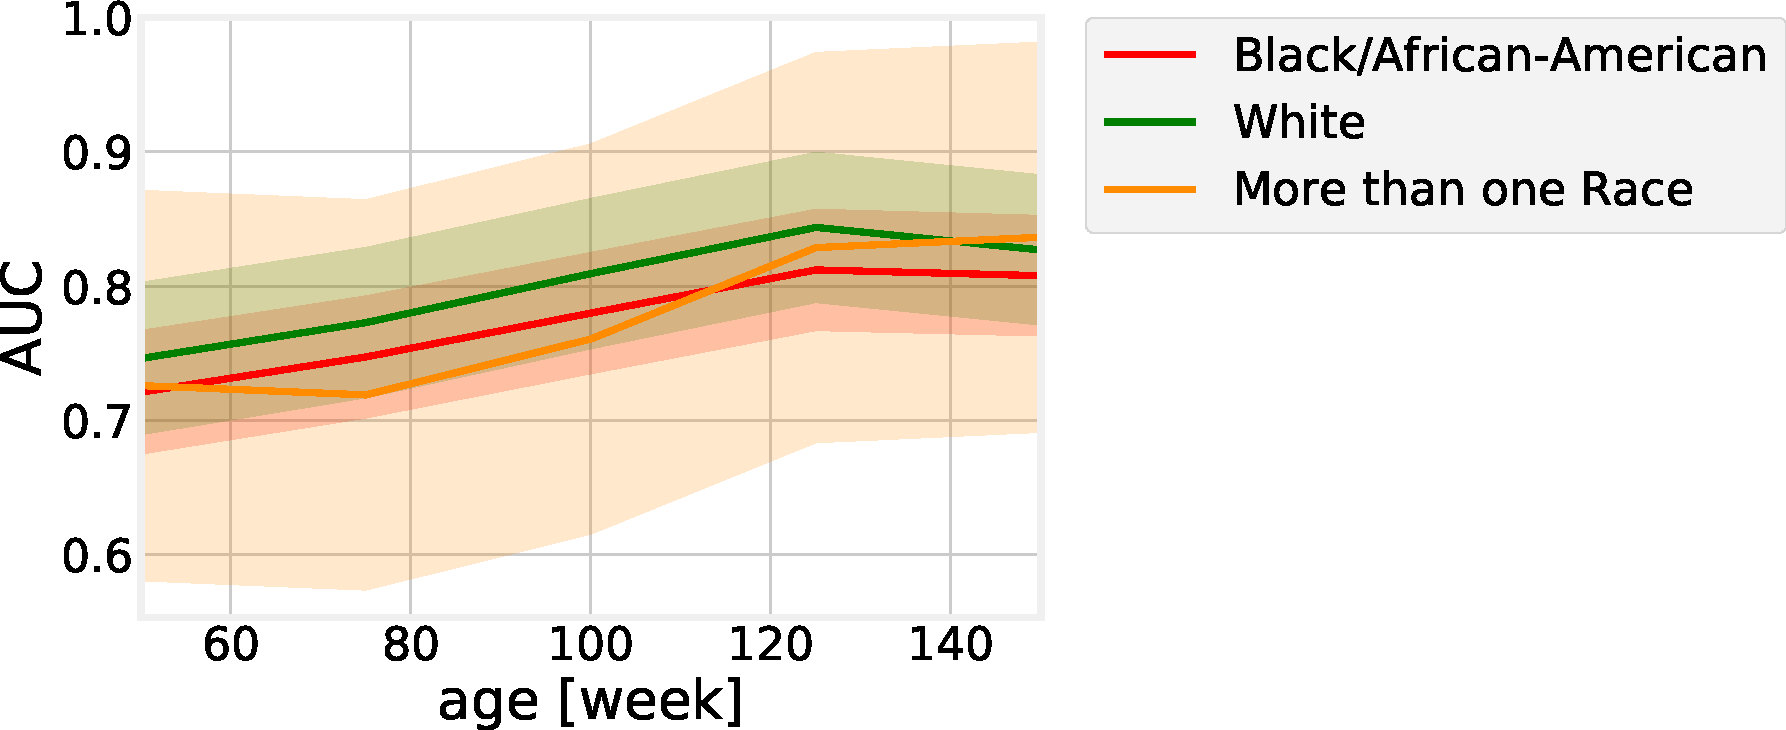
\includegraphics[height=\WDT]{../Race_M}};
\node[label={[]90:{\large A.} Female (Race) },anchor=east] (B) at (A.west) {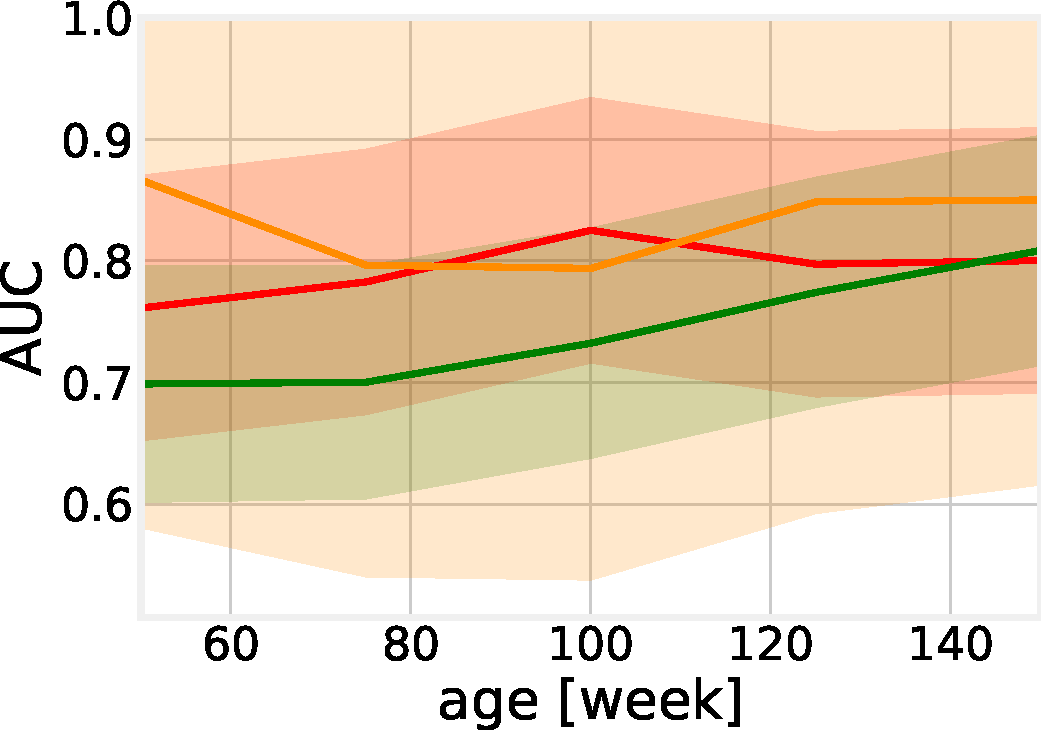
\includegraphics[height=\WDT]{../Race_F}};
\node[label={[]90:{\large C.} Female (Ethnicity) },anchor=north west] (C) at ([yshift=-.3in]B.south west) {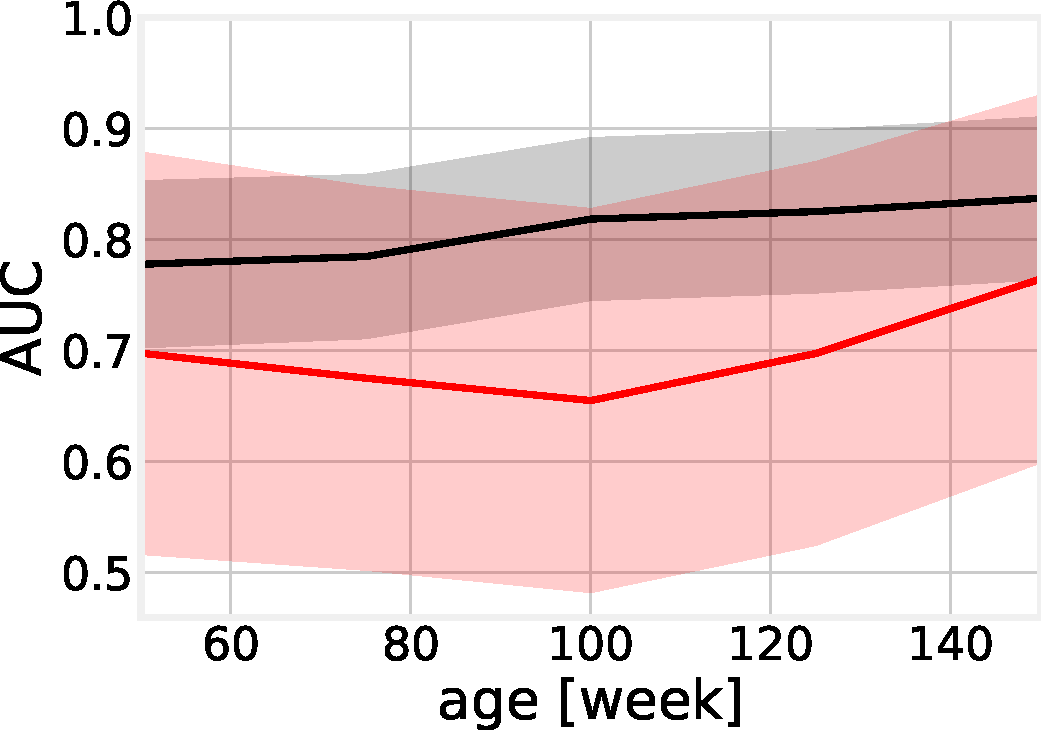
\includegraphics[height=\WDT]{../Ethnicity_F}};
\node[label={[]90:{\large D.} Male (Ethnicity) },anchor=north west] (D) at ([yshift=-.3in]A.south west) {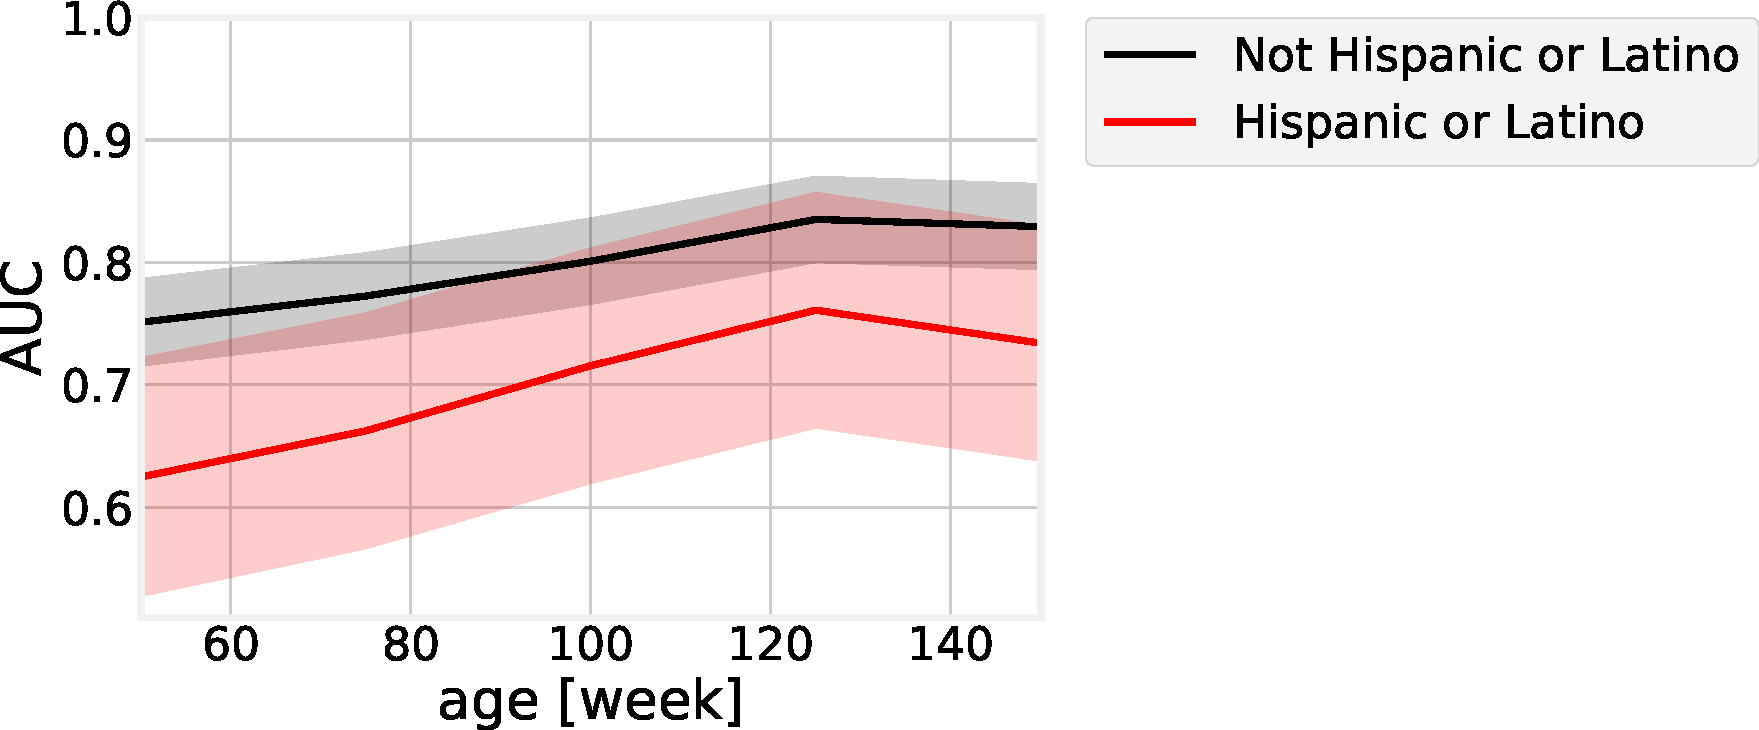
\includegraphics[height=\WDT]{../Ethnicity_M}};

  \end{tikzpicture}

\end{figure}








\end{document}



\maketitle
{  \bf \sffamily \fontsize{10}{12}\selectfont \noindent
  Alzheimer's disease (AD) represents a progressive, fatal, and incurable neurodegenerative condition, implicated as the underlying pathology in 60\%-80\% of  dementia patients, underscoring  a crucial and immediate need for effective  tools to screen for early stages of the pathology. In this study, we introduce the Zero-burden Co-morbid Risk (\zcor) score to screen for ADRD 1-10 years before a diagnosis is made under current clinical  practice. The \zcor score is  computed via sophisticated  pattern discovery on the longitudinal history of past medical encounters of individual patients, and requires  no new blood-work or cognitive tests. The rationale of leveraging incipient comorbidity signatures for early screening stems from validated or suspected mechanisms pointing to  uncharted associations existing across the human disease spectrum, $e.g.$  with psychiatric,  immunologic, endocrinal, metabolic, cardio-vascular, and other seemingly neuro-unrelated categories of dysfunctions. % Additionally, the neuropathology of ADRD appears to progress over years or decades, independently of the clinical course, implying a lengthy asymptomatic, subclinical, and/or subtly symptomatic period before ADRD is discerned. 
  Despite these suspected associations, the   current diagnostic and prognostic modalities for early AD and related dementia (ADRD) is limited, with existing tools being expensive, invasive, and sometimes inaccessible. % Imaging or cerebrospinal fluid testing for evidence of beta-amyloid plaques and neurofibrillary tau deposits, the basis for an AD classification and predictors of potential cognitive worsening,
  %is expensive, invasive, and sometimes inaccessible.
  While cognitive  assessment via questionnaire-based tools such as the Montreal Cognitive Assessment (MOCA) exist, administration is often overlooked at the primary care  visits delaying  neurology referrals, and consequently a timely diagnosis. Additionally, the efficacy of existing assessment tools in discerning especially early stages of the disease is suspect at best. In contrast, in this study, we validate the \zcor score  with over 700K patients, achieving approximately 88\% AUC  for predicting a diagnosis one year into the future, and maintaining over 80\% AUC for predictions made ten years into the future, irrespective of sex. We significantly outperform past attempts at leveraging co-morbidities. Being able to compute \zcor with little or no resource burden, implies that  we can position this as a universal screening tool,  perhaps to  be applied to entire patient populations almost instantaneously and repeatedly over time.
The \zcor score represents a new screening modality for ADRD, and can potentially identify uncharted co-morbid patterns as predictive precursors of specific ADRD presentations. Intriguing questions on the differential prevalence amongst minorities may also be investigated in this context.  % We will focus on patients aged 50+, and aim to  answer various questions, including the reliability in a prospective setting, statistical dependence if any with MOCA, the ability of co-morbid patterns to discern new  phenotypes, and investigate the underlying cause(s) for racial disparities in ADRD prevalence.
}
\vspace{15pt}



 
% \section*{Introduction}

% %Brief Project Summary & Working Hypotheses:
% Universal screening for Alzheimer’s disease (AD) based on medical health records in preclinical stages may lead to early detection of AD pathology, and to better therapeutic strategies for delaying the onset of AD. Unlike current biomarkers requiring blood-work and brain imaging, we aim to estimate risk via sophisticated pattern discovery in past medical encounters. We require no new laboratory tests, suggesting the possibility of universal AD screening in aging populations. In this study we aim to leverage at least two independent sex/age stratified medical history databases with cohort size exceeding ~600K (age: 60+ years), in order to discover subtle patterns in individual history of diagnoses, procedures, medications, with the ultimate goal of crafting a reliable estimator predicting AD 1-4 years before currently expected timeline of a clinical diagnosis. Planned research: 1) development of this predictor called Zero-burden Cormorbid Risk (ZCoR), 2) prospective validation in limited pilot trial, and 3) tentative integration within clinical workflow within a standard EHR system. Our hypotheses are: 1)  ZCoR can preempt clinical diagnosis, early enough to be clinically relevant for improving outcomes. 2) The ZCoR score correlates with AD biomarkers in current practice including CT/MRI scan abnormalities, FDG-PET, amyloid PET scans, and CSF biomarkers of A-beta, tau, and phosphorylated tau. 3) ZCoR will aid to deconfound AD disparate prevalence in older African American and Hispanic populations, and 4) deep comorbidity patterns will help characterize AD heterogeneity in a manner not possible today. 


% Past AD risk prediction models have considered predefined health variables, such as demographic, socio-economic, lifestyle and physical activity, and systolic blood pressure, BMI,  total cholesterol level and cognitive profiles . Such models are limited in their ability to account for the heterogeneous etiologies of multi-factorial AD. Standard machine learning suffer from a large data burden; specific test values (e.g. hemoglobin and urine protein levels), features and patient characteristics are needed before such models can be trained, and more importantly, applied at point of care. Our novel stochastic learning algorithm relaxes these requirements, and preliminary results show that we can reach predictive accuracies approaching 88\% ROC-AUC in identifying future AD risk 1-4 years before current clinical diagnosis. Thus translated to practice, ZCoR can significantly improve patient outcomes at little or no additional cost: ZCoR can be  computed from data already on patient file, thus making it feasible to universally screen the older population at a national level, and potentially ameliorate poor outcomes arising from late or missed diagnoses.

%\clearpage




\section*{Introduction}

Dementia may be defined as an acquired loss of cognition in one or more domains - including learning and memory, social cognition, language, executive function, complex attention, and perceptual motor function - severe enough to significantly diminish a patient's social or occupational function or both~\cite{arvanitakis2019diagnosis}. Dementia has been estimated to affect 47 million people worldwide~\cite{arvanitakis2019diagnosis}, including up to 5.5 million in the United States~\cite{owens2020screening}. Being predominantly a disease of the elderly, and given the aging of the American population, the number of dementia sufferers in the United States is projected to reach 13.8 million by 2050~\cite{as2017alzheimer}. The worldwide population of persons with dementia is expected to be over 81 million worldwide by 2040~\cite{chu2012alzheimer}. Thus there is a crucial and immediate need to find effective interventions, and tools that enable them.


The most common cause of dementia, contributing to 60\%–80\% of cases, is believed to be Alzheimer’s disease (AD), a progressive, fatal, and currently incurable neurodegenerative condition~\cite{as2017alzheimer}. Based on patient years lived with disability plus patient years lost to premature mortality, AD ranked as the $6^{th}$ most burdensome disease or injury in the United States in 2016, up from $12^{th}$ in 1990~\cite{murray2013state}. In 2018, Alzheimer's Disease and related dementia (ADRD) were the underlying cause of well over 250,000 deaths in the United States~\cite{as2017alzheimer}. ADRD also imposes a considerable burden on patients' family members and friends, estimated to include 18.6 billion hours and nearly \$244 billion in unpaid carein the United States in 2019~\cite{as2017alzheimer}.

AD neuropathology appears to progress over years or decades, independently of the clinical course, so that there may be lengthy asymptomatic, subclinical, and/or subtly symptomatic periods before ADRD is discerned~\cite{jack2018nia}. Accurate screening for both current and future cases on the Alzheimer's clinical spectrum may be expected to lead to earlier detection of AD biomarkers neuropathology and incipient cognitive impairment or dementia. In turn, such diagnostic acceleration may provide several important benefits for patients, caregivers, healthcare providers, and society~\cite{arvanitakis2019diagnosis,moyer2014screening,ahlgrim2019prodromes,patnode2020screening,borson2007implementing,davidson2019dementia}:% , albeit to date, the evidence base for these benefits,is limited~\cite{moyer2014screening,patnode2020screening}.
%
First, pharmacologic and non-pharmacologic interventions may be  applied to slow progression of cognitive impairment, while cognition is more preserved. Second, use of tailored education strategies may be facilitated to promote cognitively-impaired patients' adherence to and safe use of complex treatment regimens for comorbidities. Third, patient capacity for, and hence participation in, financial, legal, and health care decision-making may be optimized when occurring as early as possible in the syndrome's course~\cite{patnode2020screening}. Fourth, psychoeducation and case management interventions to ease caregiver burden may be proactively implemented. And lastly, patient access to clinical trials of drugs targeting cognition and dementia may be fostered, and study samples may be enriched, accelerating progress and decreasing costs of such investigations. 

% A major motivation for updating the 2011 guidelines has been the evolution in thinking about biomarkers. Studies published since 2011 have reinforced the idea that certain imaging and CSF biomarkers are valid proxies for neuropathologic changes of AD. Imaging-to-autopsy comparison studies have established that amyloid positron emission tomography (PET) is a valid in vivo surrogate for Aβ deposits (in brain parenchyma/vessel walls) [17], [18], [19], [20], [21], [22], [23], [24]. It is also now widely accepted that CSF Aβ42 (or the Aβ42/Aβ40 ratio) is a valid indicator of the abnormal pathologic state associated with cerebral Aβ [25]. An additional development has been the introduction of PET ligands for pathologic tau [26], [27], [28]. By contrast, additional research has highlighted the fact that measures of neurodegeneration or neuronal injury that are commonly used in AD research—magnetic resonance imaging (MRI), fluoro-deoxyglucose (FDG) PET, and CSF total tau (T-tau)—are not specific for AD but rather are nonspecific indicators of damage that may derive from a variety of etiologies, for example, cerebrovascular injury [29].



Current limitations of  diagnostic/prognostic modalities impeded accurate ADRD screening. While  imaging and CSF biomarkers testing for evidence of beta-amyloid plaques and neurofibrillary tau deposits have emerged recently as  valid proxies for neuropathologic changes of AD~\cite{jack2018nia} and predictors of potential cognitive worsening, such tests are  expensive, invasive, and sometimes inaccessible. Although measurement of phosphorylated tau in plasma has shown promise as a specific marker and prognostic factor for ADRD~\cite{mattsson2020longitudinal,moscosolongitudinal,karikari2020diagnostic,hall2020plasma,janelidze2020plasma}, this method is as yet unavailable in everyday practice, entails an invasive blood draw, and if widely used, may in aggregate prove costly. Neuropsychological testing instruments such as the Montreal Cognitive Assessment (MOCA)~\cite{bezdicek2020determining,Montreal87:online} have good diagnostic accuracy and some prognostic utility, but their time requirements, even when measured in minutes, may add appreciably to length-of-visit, and hence pose challenges in primary care settings~\cite{patnode2020screening,borson2007implementing}. Moreover, these instruments require validation when used in additional locales, or, especially, translated into other languages. Additionally, the efficacy of existing assessment tools in discerning especially early stages of the disease is suspect.

%Automated analysis of a patient's historic routinely-collected healthcare data may offer a non-invasive and completely passive, inexpensive, and routinely-accessible solution, with minimal time demands, to accurately discover elevated risk of


Automated analysis of a patient's historic routinely-collected health care data may offer a non-invasive and indeed, completely passive, inexpensive, and routinely-accessible solution, with minimal time demands,to accurately discover elevated risk of ADRD~\cite{wilkinson2018identifying}. The multifactorial etiologies of ADRD imply that numerous risk factors are associated with these syndromes~\cite{wilkinson2018identifying}, and administrative claims and hospital databases, due to their large or even vast scope, offer sufficient statistical power to discover exquisitely-detailed algorithms to pinpoint potential cases.  Notably, administrative claims and hospital databases may be especially amenable to exploration in heretofore unprecedented depth of associations of ADRD and comorbidities. Observational studies already have suggested that such associations encompass a large number and variety of disorders covering much of the human disease spectrum~\cite{duthie2011non}; for example, non-neuropsychiatric chronic conditions such as diabetes, hypertension, hypercholesterolemia, obesity, sleep apnea, thyroid disorders, osteoporosis, and glaucomahave been linked to ADRD~\cite{duthie2011non,anstey2020future}. The validated or suspected associations of ADRD with both ``intuitive'' categories of comorbidity, $e.g.$, neurological, psychiatric, and cardiovascular disorders, and with non-intuitive categories, $e.g.$, metabolic, endocrine, and opthalmological disorders, provide rationale for us to seek to leverage comorbid diagnoses to quantify ADRD risk.

Here we report on the development of the Zero Burden Co-morbid Risk Score (\zcor) for ADRD, which accurately identifies patients with this syndrome up to $10$ years before contemporary documented clinical diagnosis. \zcor for ADRD is a \numfeatures-feature digital signature created by applying a novel stochastic learning algorithm to perform sophisticated pattern discovery regarding relationships of comorbidities with ADRD. The training and validation cohorts for the development of \zcor included \totalpatients unique  patients, drawn from across the United States. Additionally,  \zcor for ADRD is sex stratified, with separate signatures generated for males and females. Appreciation is growing of sex/gender as a key contributor to the considerable phenotypic heterogeneity of ADRD~\cite{ferretti2020sex}, and machine learning-based analysis suggests that males and females may have different risk factors for dementia~\cite{choi2020gender}.




% Alzheimer’s disease(AD) represents a progressive, fatal, and incurable neurodegenerative condition~\cite{arvanitakis2019diagnosis,as2017alzheimer}, and   is implicated as the underlying pathology in 60\%-80\% of  dementia cases. The neuropathology of AD and related dementias (ADRD) appears to progress over years or decades, independently of the clinical course, implying a lengthy asymptomatic, subclinical, and/or subtly symptomatic period before ADRD is discerned~\cite{jack2018nia}. One barrier to accurate screening for  ADRD or cognitive impairment signaling early stage AD, is the limitation of current diagnostic and prognostic modalities. Imaging or cerebrospinal fluid testing for evidence of beta-amyloid plaques and neurofibrillary tau deposits, the basis for an AD classification~\cite{jack2018nia} and predictors of potential cognitive worsening, is expensive, invasive, and sometimes inaccessible. While cognitive  assessment via questionnaire-based tools such as the Montreal Cognitive Assessment (MOCA) exist, administration is often overlooked at the primary care  visits delaying  neurology referrals, and consequently a timely diagnosis. Additionally, the efficacy of existing assessment tools in discerning especially early stages of the disease is suspect at best. With the number of dementia sufferers in the United States  projected to reach 13.8 million by 2050~\cite{as2017alzheimer,moyer2014screening,owens2020screening},  there is a crucial and immediate need to find effective interventions, and tools that enable them.

% In this study we resport  a novel reliable approach to  screen for ADRD up to 10 years in the  future, enabled by learning algorithms that   analyze deep comorbidity patterns emerging in the longitudinal history of past medical encounters of individual patients. Focusing on patients aged 50+, we engineer a sex-stratified  risk estimator, known as the Zero Burden Co-morbid Risk Score (\zcor) score, which may be computed with no new blood-work or cognitive tests. Our rationale stems from validated or suspected mechanisms pointing to  uncharted co-morbid associations existing across the human disease spectrum, $e.g.$  with psychiatric,  immunologic, endocrinal, metabolic, cardio-vascular, and other seemingly neuro-unrelated categories of dysfunctions~\cite{duthie2011non,anstey2020future,newcombe2018inflammation,van2016genetic,tortajada2020prevalence} that we leverage to quantify risk. Early diagnosis  enables pharmacologic and non-pharmacologic interventions  to slow  cognitive decline, improving quality of life,  easing caregiver burden, and offering more chances to participate in new clinical trials, in turn enriching study samples that improve odds of finding better therapeutics towards an eventual cure.






% Alzheimer’s disease(AD) represents a progressive, fatal, and currently incurable neurodegenerative condition3, and currently  is implicated as the underlying pathology for 60\%-80\% of  dementia patients.  Based on patient years lived with disability plus patient years lost to premature mortality, AD  ranked as the 6th most burdensome disease or injury in the United States in 2016, up from 12th in 19904, and  Alzheimer’s dementia and related disorders (ADRD) nationally contributed to well over 250,000 deaths3 in 2018. ADRD also imposes a considerable burden on patients’ family members and caregivers, as exemplified by  18.6 billion hours of commitment, and nearly \$244 billion in unpaid care in the United States alone in 20193.


% {\color{Red2} AD treatment is complicated, and delayed diagnosis severely impacts patient outcomes.} AD neuropathology appears to progress over years or decades, independently of the clinical course, so that there may be a lengthy asymptomatic, subclinical, and/or subtly symptomatic period before ADRD is discerned5. Accurate screening for both current and future cases on the Alzheimer’s clinical spectrum may be expected to lead to earlier detection of AD biomarkers and incipient cognitive impairment or dementia. In turn, such diagnostic acceleration is expected to significantly improve patient outcomes, and positively impact caregivers and  healthcare providers1,2,6-9.

%[DISCUSSION]
%First, pharmacologic and non-pharmacologic interventions may be promptly applied to slow progression of cognitive impairment, while cognition is more preserved. Second, use of tailored education strategies may be facilitated to promote cognitively-impaired patients’ adherence to and safe use of complex treatment regimens for comorbidities. Third, patient capacity for, and hence participation in, financial, legal, and healthcare decision-making may be optimized when occurring as early as possible in the syndrome’s course7. Fourth, psychoeducation and case management interventions to ease caregiver burden may be proactively implemented. Lastly, patient access to clinical trials of drugs targeting cognition and dementia may be fostered, and study samples may be enriched, speeding completion and decreasing costs of such investigation.  

% One barrier to accurate screening for current and future ADRD is the limitations of current diagnostic and prognostic modalities. Imaging or cerebrospinal fluid testing for evidence of beta-amyloid plaques and neurofibrillary tau deposits, the basis for an AD classification5 and predictors of potential cognitive worsening, is expensive, invasive, and sometimes inaccessible. Although measurement of phosphorylated tau in plasma has shown promise as a specific marker and prognostic factor for ADRD10-14, this method is as yet not commonly available in clinical  practice, entails an invasive blood draw, and if widely used, may in aggregate prove costly. Neuropsychological testing instruments have good diagnostic accuracy and some prognostic utility, but their time requirements, even when measured in minutes, may add appreciably to length-of-visit, and hence pose challenges in primary care settings7,8. Moreover, these instruments require validation when used in additional locales, or, especially, translated into other languages.
  

% Automated analysis of a patient’s historic routinely-collected healthcare data may offer a non-invasive and indeed, completely passive, inexpensive, and routinely-accessible solution, with minimal time demands, to accurately discover elevated risk of ADRD15. The multifactorial etiologies of ADRD imply that numerous risk factors are associated with these syndromes15, and administrative claims and hospital databases, due to their large or even vast scope, offer sufficient statistical power to discover exquisitely-detailed algorithms to pinpoint potential cases.  Notably, administrative claims and hospital databases may be especially amenable to exploration in heretofore unprecedented depth of associations of ADRD and comorbidities. Observational studies already have suggested that such associations encompass a large number and variety of disorders covering much of the human disease spectrum16.   

% Here we report on the development of the sex stratified Zero Burden Co-morbid Risk Score (ZCoR) for ADRD, which accurately screens for  patients  up to 10 years before contemporary documented clinical diagnosis. ZCoR for ADRD is a \numfeatures-feature digital signature created by applying a novel stochastic learning algorithm to perform sophisticated pattern discovery, with the aim  to exploit known and possibly   uncharted relationships of comorbidities with ADRD. The \zcor score may be computed simply from the history of medical encounters for individual patients, and requires no new blood-work or  laboratory tests, and maybe administered universally to aging populations. Universal screening, in addition to its obvious impact, can help illuminate the source of  demographic and ethnic disparities in AD prevalence~\cite{matthews2019racial}. Thus, expected to be widely, readily, and  rapidly  applicable at points of care, the \zcor tool can  impact outcomes by reducing missed diagnoses and  diagnostic delays, and significantly accelerate the diagnostic time-line, all with little or no additional burden on the patient, caregiver, or healthcare resources. Notably, administrative claims and hospital databases may be especially amenable to exploration in heretofore unprecedented depth of associations of ADRD and comorbidities. Observational studies already have suggested that such associations encompass a large number and variety of disorders covering much of the human disease spectrum16. 

  
%The training and validation cohorts for the development of ZCoR is substantial,  exceeding 700,000 patients in total. 


%The sex stratification pf \zcor yields  distinct  signatures  for males and females. Appreciation is growing of sex/gender as a key contributor to the considerable phenotypic heterogeneity of ADRD16, and our analysis corroborates that males and females may be differentially impacted by risk factors for dementia17. 


\section*{Materials and Methods}
\subsection*{Data Source \& Patient Selection}
%
Our patient data  comes from  the Truven Health Analytics MarketScan\textsuperscript{\textregistered} Commercial Claims and Encounters Database for the years 2003-2018~\cite{hansen2017truven} (referred to  as the Truven dataset). This US national database merges  data contributed by over 150 insurance carriers and large self-insurance companies,  and comprises over  seven billion time-stamped diagnosis  codes. The entire database tracks over  \numTruven patients for 1 to 15 years,  reflecting a substantial cross-section of the US population. We select our cohort(s) from the Truven dataset in accordance with the inclusion/exclusion criteria described in  Table~\ref{tabpreex}, ensuring that selected patients haveat least  three years of  medical history recorded in the dataset. The geographical distribution of the patients in our selected cohort(s) is illustrated in Fig.~\ref{figdesc}a. Fig.~\ref{figdesc}b illustrates the age distribution at the time of \DISEASE diagnosis (mean $\approx 68$ years), which is consistent with the reported mean onset age for \DISEASE ($\approx 66$ years~\cite{ley2011a}). We also note that observed risk of onset actually increases with age, which is computed as the number of \DISEASE cases normalized by the total  number of patients at the same age, as shown in Fig.~\ref{figdesc}c.

Predicting  future ADRD diagnosis   is a  binary classification problem: we classify time-stamped sequences of diagnostic codes  into \treatment and \control categories, where the ``\treatment'' category refers to patients  diagnosed with ADRD at  $\PREDWINDOW$ year from the point of screening (one or more codes mapping to ADRD appears in record shown in Table~\ref{tabtarget}, referred to as the Dx problem in Table~\ref{tabres}) or are identified by either such codes or prescription of  AD related medication~\cite{FDAAppro97:online,park2020machine} (Donepezil, Galantamine, Memantine or Rivastigmine, referred to as the Dx/Rx problem in Table~\ref{tabres}). We also consider  earlier screening up to $M$ years before the actual diagnosis, with the \control cohort comprising patients with no indication of ADRD in $M+2$ years in future; we investigated values of $M=0,\cdots,10$, $i.e.$, predicting ADRD immediately before a clinical diagnosis to up to a decade in the future. The control cohort comprises patients who never develop AD, $i.e.$, do not have ADRD target codes and are ever prescribed AD related medication. We base our predictions on the past $\INFWINDOW$ years of diagnostic history. Overall we analyze $n=\totalpatients$ patients, with $\totalnpos$ patients in the \treatment group and $\totalnneg$ patients in the \control group (See CONSORT diagram in Fig.~\ref{fig0}c), considering approximately  42 million diagnostic codes, with over 46K unique codes in total for both sexes.

We do not pre-select any diagnostic   code based on its  suspected comorbidity with ADRD. To investigate if our  performance changes substantially for ``high risk'' patients identified  based on known co-morbidities including  obesity, type II diabetes mellitus, hypertension, atherosclerosis, atrial fibrillation,  dyslipidemia, depression, alcohol abuse, and pneumonia, we   separately consider high risk and  low risk sub-cohorts. The high risk sub-cohort comprises patients with one or more of the diagnoses enumerated in Table~\ref{tabhirisk}, which identify the top known co-morbidities~\cite{tortajada2020prevalence,duthie2011non}.  The low risk sub-cohort comprises  patients who are not at high risk as specified by  the previous condition.
Results in the low risk sub-cohort is of particular significance; these patients are at a higher risk of  missed diagnosis.

\subsection*{Modeling \& Prediction}
The significant diversity of diagnostic codes, along with the sparsity of codes per patient (approximately one entry every 100 steps on the diagnostic time series, see below)   makes this a difficult learning problem. % {\color{Red1} Our results demonstrate that performance from  off-the-shelf classifiers such as random forests, gradient boosting and deep learning may be superseded by stochastic learning algorithms  customized for pattern discovery in diagnostic sequences.}
We proceed by  partitioning the  disease spectrum into \DXphn\xspace broad  categories, $e.g.$ infectious diseases, immunologic disorders, and endocrinal disorders (See SI Tab.~\ref{SI-tabicd}  for a detailed enumeration of these categories). Some of these categories comprises a relatively large number of diagnostic codes aligning roughly with the  categories defined within the ICD framework~\cite{world1988international}.    Each of the diagnostic categories yield a single time series over weeks (each week being identified as having a value '0' for no code corresponding to the diagnostic category, or  '1' if some code is present, and '2' if a diagnostic code from any of the other categories is present). We have \avgNumDX diagnostic codes  per broad category per patient per week, implying that these event streams have one  entry specific to the represented set of disorders every 100 steps on average.

%2\times\RXphn=\the\numexpr \DXphn + 2*\RXphn \relax
We refer to the individual diagnostic categories  as a  phenotype in the sequel, since they are  observable characteristics of the patients.  Once we have defined  these diagnosis phenotypes, each patient is  represented by $\DXphn$  sparse  stochastic time series of  events, which  are  compressed into specialized Hidden Markov Models known as Probabilistic Finite Automata~\cite{CR08,CL12g}. These models are inferred separately for each phenotype,  for each sex, and for the control and the \treatment cohorts,  to identify  the distinctive average patterns  emerging at the population level. Thus, we infer 
$\DXphn\times 2 \times 2  = \the\numexpr  \DXphn  *2 *2  \relax$  PFSA models in total in this study. Our inference algorithm (See Supplementary Text, Section~\ref{SI-sec:PFSA}))  for these models do not presuppose a fixed structure, and is able to work with non-synchronized and variable length data streams. Variation in the structure and parameters of these inferred models between the \treatment and \control groups  delineate the estimated risk of an \DISEASE diagnosis at the population level. Given these models, and  the history of a specific patient, we can then quantify the likelihood of this patient's particular history being generated by the \control PFSA models as opposed to the \treatment models. We refer to this likelihood difference as the sequence likelihood defect (SLD)~\cite{huang2019data}, which is the one of the key informative features in our approach. The SLD is a  novel concept, involving the generalization of the notion of KL divergence~\cite{cover} between probability distributions to a generalized divergence between possibly non-iid stochastic processes (See Supplementary Tex, Section~\ref{SI-step2}). 
 
{\color{Red1}
In addition to the phenotype specific Markov models, we use a range of engineered features that reflect various aspects of the patient-specific diagnostic histories (referred to as the ``sequence features''). These  include the ratio of number of weeks with the codes of a given phenotype to the total number of weeks in sequence, the ratio of number of weeks with the codes of a given phenotype to the number of weeks with any diagnosis code recorded and the length of the longest uninterrupted subsequence of weeks with the codes of a given phenotype (See Table~\ref{tabfeatures} for complete list of such features). Ultimately, we compute a total of $\numfeatures$  features    for each patient, which is then used to train a standard gradient boosting classifier~\cite{ke2017lightgbm} aiming to  map   individual patients  to a raw risk score. We randomly choose  $75\%$ of our patients for training with the rest  held-out as a validation set. $50\%$ of the training data is used for PFSA inference, and the rest for training the  gradient boosting classifier.}

\subsection*{Raw Risk \& Relative Risk}
Our predictive pipeline produces a continuous estimate of the raw risk score of an \DISEASE diagnosis in future. Thus, our raw risk estimate is a continuous number, and  we must choose  a decision threshold to make crisp predictions,  $i.e.$, if the raw risk is greater than this calibrated threshold then the individual patient is predicted to be in the \treatment category. In this study, we select this threshold by maximizing the $F_1$-score, defined as the harmonic mean of sensitivity and specificity, to make a   balanced trade-off between Type 1 and Type 2 errors. The \textit{relative risk} is then defined as the ratio of the raw  risk to the  decision threshold, and a value  $>1$  indicates  a predicted  future \DISEASE diagnosis.

\subsection*{Performance Measurement}
We measure our performance using  standard metrics including the Area Under the receiver-operating characteristic curve (AUC), sensitivity, specificity and the Positive Predictive Value (PPV). We also report accuracy (acc, See Table~\ref{tabperf}), which is the probability  of a  correct prediction (\treatment or \control).

\subsection*{Feature Importance \& Comorbidity Spectra}
Beyond the demonstrated predictive performance (see Results), calculation of the \pcor score offers  insights into the comorbid associations of \DISEASE that might actually have predictive value. Estimating the relative importance of the features used is crucial for  sanity checks, as well as  for insights into the underlying causal mechanisms. We compute the relative importance of the features  by estimating the  mean change in the raw risk via random perturbation of a particular feature: this is the ``feature importance'' shown in Fig.~\ref{fig0}c for the different diagnostic categories.  which  illustrates that respiratory disorders are the most important diagnostic category modulating the \pcor score. 

Importantly, all of  our features are  based on data already  available in the past  medical records. We do not demand results from specific tests, or look for specific demographic, bio-molecular, physiological and other parameters; \textit{we use what we get} in the diagnostic history of patients, which presents un-structured sequence of labels pertaining to the ICD and the prescription codes, and is typically prone to noise, coding errors and sparsity. Our ability to effectively work with uncurated data and  achieve high out-of-sample predictive performance   showcases the  immediate clinical  applicability with zero additional burden to patients and providers.

In addition to the patient-specific predictions, we compute
the statistically significant log-odds ratio of specific ICD codes occurring in the true positive vs the true negative patient sets. We call these the comorbidity spectra (See Fig.~\ref{figspecA}). Removing the false positives and the false negatives from consideration in computing the comorbidity spectra allows us to uncover patterns | at the level of individual codes | that are most representative of the patient risk. Importantly, the comorbidity spectra are based on individual codes, as opposed to the feature importances shown in Fig.~\ref{fig0}c, which consider aggregated impact of all features that are based on the broad disease categories. Every disorder listed in the co-morbid spectra obviously do not all appear in a single patient, but the idea here is that the codes with high log-odds ratio are  significantly more likely in \treatment cohort. The comorbidity  spectra, so named because of disease-category specific  color coding, offers unique  insight into the predictive   co-morbidity burden of \DISEASE.



\section*{Results}
In this study we demonstrate three key results: 1) high out-of-sample predictive performance for identifying a future \DISEASE diagnosis via leveraging subtle comorbidity patterns recorded in the past medical history of individual patients.  2) the ability of our models to  maintain high predictive performance for an  eventual diagnosis further into future, upto 10 years. And 3) ability to perform effectively for both low and high-risk cohorts, such as a preexisting diagnosis of COPD, asthma or  heart disease, or the absence of any indication of dyspnea in the past.

Our main prediction results are presented in Fig.~\ref{fig0}a-b, which illustrate the ROC and the precision-recall curves respectively (for screening one year before current diagnosis), shown separately for males and females. As noted in the legend of these panels, our out-of-sample predictive performance is  $>88\%$ AUC irrespective of the sex of the patient, with $>55\%$ sensitivity at $95\%$ specificity ($55\%$ for males and $60\%$ for females). At $99\%$ specificity, we obtain a positive predictive value (PPV) of $52\%$ for females and $54\%$ for males, with sensitivities at $42\%$ and $38\%$ respectively. At these values we obtain an accuracy 
of $\approx 94-98\%$ (See Table~\ref{tabres}) which indicates the overall fraction of correct predictions. The PPV achieved by \zcor at maximum accuracy is $70\%$ for females and $71\%$ for males, with a corresponding Negative Predictive Value (NPV) of $98\%$.

%
%We achieve accuracies $>95\%$ (See Table~\ref{tabres}), which indicates the overall fraction of correct predictions. We achieve a PPV of  $5-6\%$, which compares favorably with the maximum theoretical value of $\approx 9\%$  at  $95\%$ specificity, given the low population prevalence of \DISEASE  at $0.004945$ in the US~\cite{sauleda2018idiopathic}.

Thus, to summarize: our predictive pipeline detects about 55-60  out of every 100 patients who are going to have a diagnosis in 1 year, if we operate at $95\%$ specificity. If we wish to operate at the higher specificity of $99\%$, then out of 100 positive flags we have about 50-52 true positives.  The accuracy metric indicates that  we are correctly identify  the risk status (\treatment or \control) for approximately  94-98 out of 100 patients, irrespective of sex, highlighting the potentially high clinical significance of the \zcor score.

From  the inferred  relative importance of the  features (See Fig.~\ref{fig0}d-e), we conclude, as expected, that respiratory disorders  in the past are the most important modulators of risk, followed by known or suspected \DISEASE comorbidities, metabolic  diseases, cardiovascular abnormalities and diseases of the eye. Infections also feature  in the top 20 co-morbidities shown in these panels. Importantly while there are sex differences, the overall pattern of the relative importance ranking remains substantially invariant between males and females. With some exceptions, many of these patterns are not particularly surprising; the contribution of this study is to bring them  together systematically to realize an  accurate risk estimate via the \zcor score.

A key metric to evaluate the potential impact of the \zcor score is to estimate the expected change in the survival functions via a Kaplan-Meyer (KM) analysis~\cite{kaplan1958nonparametric}, and the corresponding change in the mean survival time. The standard KM analysis is specifically designed  to handle scenarios with incomplete observations, $e.g.$ not knowing the exact time of death for all patients, but merely a lower bound on their survival times. This is particularly useful in our case, since we found that  insurance claims often do not record deaths, with expired patients  simply dropping off the database. This creates uncertainty on if the patient had actually expired, or if he or she simply dropped insurance, or got dropped from the database for  some other reason. Nevertheless, the time over which they are observed in the database is clearly a lower bound on their survival. With this mind, we construct the survival plots shown in Fig.~\ref{figKMF1}a-b, which represents lower bounds on the survival function (panel a) and upper bounds on the hazard rate (panel b), shown along with 95\% confidence bounds. Note that since we can operate our predictors at different specificity-sensitivity trade-offs, we get different curves if we vary the specificity. The survival functions are notably similar across the two sexes. Panel c shows the variation of lower bound on the  mean survival times, compared with the baseline currently observed in the database; even at 95\% specificity we boost the lower bound on mean  survival time from around 100 weeks to approach 180-200 weeks. It is crucial to note that these survival analyses do not take int account the possibility of actually prolonging life via clinical interventions when we push back the time of the  diagnosis; thus in actuality we expect the survival times to be markedly better to what is shown in Fig.~\ref{figKMF1}a-c.

Our predictive performance expectedly degrades as we predict earlier, and this is illustrated in Fig.~\ref{figKMF1}e. Importantly however, the degradation is slow enough that we can use \zcor with acceptable reliability to predict diagnoses four years into the future. To illustrate how the \zcor risk varies over patient age, we estimate the distribution of the scores over the \treatment and the \control cohorts in Fig.~\ref{figKMF1}d. Note that for patients fore who get eventually diagnosed, the risk almost linearly increases with age. 

While these results demonstrate the importance of the  diverse features used in our approach, understanding the seat of this predictive power is important. The feature importances discussed earlier (Fig.~\ref{fig0}d-e) identify the relative impact of broad disease categories. Importantly, to evaluate the feature importance of a specific diagnostic category,  we sum the importance of all  features  based on that  category, not just the presence or absence of individual diagnoses. The latter aspect is investigated via the co-morbidity spectra for out-of-sample patients, shown in Figs.~\ref{figspecA} separately for males and females.  We find that the important co-morbidities are diverse, vary with the sex of the patients, but is clearly dominated by respiratory disorders, followed by diseases of the cardiovascular and circulatory systems. Again, while many of these patterns  are expected at the population level, design of the personalized \zcor score is not immediately obvious.

Since \DISEASE co-morbidities have been investigated in the literature, a relevant question here is if our performance is dramatically better in sub-cohorts defined by the presence of these high risk diagnoses in the past (defined in Table~\ref{tabhirisk}). The results are tabulated in Table~\ref{tabres}, showing that our performance in the high risk sub-cohort is more or less comparable  with full cohort performance. The AUCs achieved for the low risk cohort is somewhat lower ($> 85\%$ for males and females), but still acceptably high. % The ROC and the precision-recall curves for the low risk sub-cohort is shown in Fig.~\ref{fig0}a-b, where we note that our sensitivity drops to $48\%$ at 95\% specificity, with the PPV dropping slightly to $4.6\%$.
Thus, even within the low risk patients, we still detect 48  out of every 100 patients who are going to have a diagnosis in 1 year.% , and out of 100 positive flags we have about 5 true positives on average. And our accuracy in this cohort is still about $95\%$, so as before, our decision is wrong in the case of less than 5 out of every 100 patients.

\section*{Discussion }

This report describes the development, using a vast US commercial claims database, the validation, using a large urban academic medical center database, and the predictive performance, using both cohorts, of the ZCoR automated digital screening tool for ADRD syndromes. Our key observation was that in both men and women $\geqq 50$ years old seen in diverse community or academic settings during 2003-2018 (n=341,318, n=387,700, respectively), ZCoR could accurately detect ADRD clinical spectrum cases up to 10 years before diagnosis was first documented. At 10 years before documented diagnosis, ZCoR would have predicted ADRD with an AUC approaching 80\%, at 3 years before documented diagnosis, with an AUC of 87\%, and at 1 year before documented diagnosis, with an AUC approaching 88\% (Fig. ?, Table ?, Supplementary Table ?). Notably, because beyond the patient’s sex, ZCoR considers only diagnostic data already in his/her electronic medical record, and because ZCoR runs on existing information technology infrastructure, the digital signature operates non-invasively, inexpensively, and nearly instantaneously, and is potentially very widely, if not universally accessible. ZCoR encapsulates sophisticated, automated, fully data-driven pattern discovery of cormorbidities as ADRD risk factors, weighing 671 features related to the incidence, timing, and sequence of individual diagnostic codes, with stratification by sex. Hence in everyday practice, ZCoR would add the novel dimensions of comorbidity and sex to supplement the other demographic, neuropsychological, functional, biofluid measurement, and imaging tools currently informing assessment of patients’ likelihood of having or developing ADRD. Notwithstanding ZCoR’s novelty, our findings of cardiovascular, ischemic, psychiatric, neurological, and metabolic disorders as among the most important illness categories associated with ADRD in either sex align with relationships between these factors and the target condition that already have been documented via machine learning15-17 and observational studies18, lending credence to ZCoR accuracy. Also lending such credence is the score’s acknowledgment, via sex-stratification, of differences between males and females in ADRD risk factors, natural history, and symptoms14,15,19-23. 

To our knowledge, ZCoR is one of three digital signatures for ADRD reported since 2020, joining those of Boustani et al, developed utilizing data from the Indiana Network for Patient Care16, and of Park et al., developed utilizing data from the Korean National Health Insurance Service17. Although the respective reported prognostic timeframes are not fully comparable, our digital signature appeared to achieve the best performance of the three (Supplementary Table XX). Notably, the AUC of ZCoR for ADRD at 10 years before documented diagnosis surpassed the AUCs of the Boustani et al. signature for the 1–10-year, 3–10-year, or 5–10-year before diagnosis timeframes by ?\%–?\% on an absolute basis, and ?\%–?\% on a relative basis. Also of interest, for each annual timepoint 0–4 years before documented diagnosis, the AUCs of ZCoR for ADRD exceeded those of the Park et al. signature by ?\%–?\% on an absolute basis, and ?\%–?\% on a relative basis. 

A number of methodological differences may have contributed to these respective performances. First, and in our opinion most importantly, [summary of how/why your “special sauce algorithm” is better]. Second, in contrast to the other signatures, ZCoR for ADRD was stratified by sex, and as noted, our work and that of others15 using “data mining” suggest that indeed, ADRD risk factors differ appreciably in males versus females. Third, our algorithm was derived using a cohort roughly 10–18-fold larger than those of Boustani et al. or Park et al: 729,018 versus 40,736 or 71,466. In other words, our pattern discovery could capitalize on magnitudes larger quantities of data. Fourth, unlike that of Boustani et al. (but like that of Park et al.), our algorithm was completely data-driven; instead, the Indiana investigators used expert opinion-generated variables in the first phase of developing their digital signature. Using only data-driven algorithms may most fully leverage the ability of machine learning to discern subtle patterns in vast amounts of data, while minimizing bias. Fifth, again unlike Boustani et al (but like Park et al.), we considered only structured data, i.e., ICD codes, and not the possibly more subjective healthcare provider notes in the medical record. Lastly, unlike those of our conterparts, our analysis weighed only comorbidities and sex, not other demographic factors, treatment-related factors, or testing-related factors (e.g., race, medication, or laboratory results). We chose to use only structured data on comorbidity, as well as sex, in the interest of optimizing availability of the information in, and hence, scalability to, everyday practice. As well, inclusion of prescription information in our algorithm appeared not to improve performance (data not shown). 

We envision three main potential applications of ZCoR for ADRD. First, the score can serve in primary care or specialist settings (e.g., neurology, gerontology) as a screening tool for future incident overt cases, with the potential diagnostic, therapeutic, psychosocial, caregiver-related, and research benefits noted in the introduction to this paper. ZCoR could, for example, be routinely deployed, alone or along with a brief, validated neuropsychological instrument, as recommended by the American Academy of Neurology (\url{https://www.aan.com/Guidelines/home/GuidelineDetail/881}, accessed 9 February 2021), in the cognitive screening mandated since 2011 as part of the Medicare annual wellness visit.4 Alternatively, especially given the variable clinical natural history of such patients24, ZCoR could be employed in individuals with subjective memory decline but largely-intact cognition and function, or in those with incipient mild cognitive impairment, e.g., worsening but still personally-appropriate serial neuropsychological test scores, who have not undergone biofluid or imaging assessment for ADRD-related or other dementia-related pathology. Notably, from pharmacoeconomic, practical, and psychosocial standpoints, use of ZCoR for “long-range” clinical prognostication may be compatible with the up-to-decades-long, pre-clinical progression of beta-amyloid and tau neuropathology in ADRD: even 10 years before overt cognitive impairment, biofluid testing or imaging performed due to ZCoR high-risk status is likely to be informative7, and the ZcoR classification, actionable. 

A second potential ZCoR application could be screening for undiagnosed prevalent cases of ADRD in primary care settings. Considering the estimated 45%–80% of dementia cases in older adults that go undiagnosed in the US25, availability of a non-invasive, inexpensive, near-instantaneous, and almost universally-accessible tool could revolutionize detection of such patients. 

Third, ZCoR could be applied in scientific research regarding ADRD natural history and prevention. Beyond enrichment of trials of prophylactic interventions against cognitive impairment, ZCoR opens intriguing avenues of investigation, e.g., examination of the roles of previously-underrecognized comorbidity classes with important associations with ADRD, e.g., musculoskeletal disorders in males,  respiratory infections in females, reproductive or ophthalmological disorders in both sexes. 

Strengths and limitations of the present work merit consideration. Chief among the former is the development of an accurate, practical, long-term screening tool capitalizing on and systematizing arguably underutilized dimensions of ADRD assessment, namely, comorbidities and sex 14,18. Chief among the limitations may be the known disadvantages of administrative claims databases, in particular, potential diagnostic miscoding, a situation that might be exacerbated by the current frequent imprecision in Alzheimer’s-related nomenclature7. It might be argued that coupled with the high prevalence of undiagnosed dementia, mis-coding could lead to our ADRD signature deriving from data of only a fraction, albeit a substantial fraction, of our true cases. This situation might pose a particular peril under our “probable ADRD” definition considering only diagnostic codes, and not prescriptions of anti-dementia medication. Mitigating this concern are the vast size of our control groups (n=375,101 females, n=375,101 males) and the limited population prevalence of ADRD even were undiagnosed cases counted; these two factors imply that “non-signal” from large numbers of “true controls” is likely to overwhelm “buried ADRD signal” from “false controls”. An additional possible concern related to mis-coding would be inclusion of non-ADRD dementia cases among the ADRD group. Arguably mitigating this concern somewhat is the “mixed” picture of the dementia afflicting many patients with ADRD2,7.  The mixed profile would make characteristics of patients with non-ADRD cognitive impairment also pertinent to many patients with the target condition. One could additionally assert that our screening tool might have been stronger had we included treatment-related factors, e.g., medications, along with comorbidities. As noted, however, using only diagnostic codes may increase the availability of data inputs for ZCoR in everyday practice, and hence the tool’s scalability to and generalizability to routine settings. Moreover, comorbidity codes may be viewed to at least some extent as surrogates capturing the effects of medications that might influence Alzheimer neuropathology, e.g., statins or anti-diabetic agents, at the same time that they capture the effects of the comorbidities themselves. 

It is worth acknowledging that early detection of progressive, not-yet-well-manageable brain disorders that have major effects on capacity, autonomy, and healthcare and other resource utilization, poses potential risks as well as rewards1. These risks include stigmatization and discrimination. It will be necessary to further explore these and other potential harms of early recognition of Alzheimer cognitive impairment, and to seek their amelioration through legal and public health policy changes1,4. 

Moving forward, our focus for additional research regarding ZCoR for ADRD includes: 1) prospective validation and proof-of-concept in a limited pilot trial of routine application of the signature; 2) assessment of the effects of ZCoR use on patient and caregive quality-of-life, patient cognition and function, and healthcare utilization; 3) correlation with ADRD clinical and neuropathological biomarkers such as neuropsychological and functional test results and biofluid and imaging findings related to beta-amyloid, tau, and neurodegeneration; 4) comparison of ZCoR performance in different racial groups and ethnicities, including examination of the signature’s ability to reduce disparities in the rate of diagnosis.   

\section*{Conclusion }

We developed and validated ZCoR for ADRD, a screening tool capable of detecting with high accuracy patients with Alzheimer cognitive impairment as long as 10 years before an ADRD diagnosis was documented in everyday community and academic practice throughout the United States. By analyzing comorbid patterns in a systematic and automated fashion, and by acknowledging sex differences in AD and ADRD, ZCoR may for the first time provide clinicians and researchers with the means to incorporate under-utilized dimensions into ADRD risk assessment. In so doing, ZCoR would open new avenues in identification of and intervention against cognitive impairment, as well as neurocognitive research and caregiver support. Additionally, ZCoR would supplement the neuropsychological and functional testing, biofluid measurement, and imaging that currently form the mainstays of dementia diagnosis and prognostication. ZCoR runs on contemporary information technology infrastructure, and can operate inexpensively and nearly instantaneously at the point of care. Hence ZCoR holds promise as a routine screening tool for primary care practitioners, gerontologists, neurologists, psychiatrists, and psychologists to use in middle-aged or elderly patients, particularly individuals with early signs of cognitive impairment, or age-related, lifestyle-related, or family-related risk factors for that condition. The effects of ADRD screening using ZCoR on the accuracy and speed of diagnosis, on health care resource utilization, and eventually, on patient and caregiver outcomes, warrant prospective study.  
   
\bibliographystyle{naturemag}
\bibliography{ad,ipf,aut,bipolar,BibLib1}

\input{figuresandtables}
\end{document}

% ############################################
% ############################################
% ############################################
% \begin{figure}
%   \tikzexternalenable
%   \tikzsetnextfilename{KMF1}
%   \centering
 
% \input{Figures/figsurvival}
% %/run/media/ishanu/D3/pub_pf_/data/SURVIVAL
% %/run/media/ishanu/D3/pub_pf_/data/MVP_PREDS/offset_performance.csv 
%   \captionN{\textbf{Survival function, hazard rate improvements, prediction horizons and peformance in low-risk sub-cohorts.} \textbf{Panel a} shows the estimated lower bounds on the survival function at two specificity levels (90 and 95\%), and \textbf{panel b}  the estimated upper bounds on hazard rates. The lower (upper) bounds are estimated due to the often missing information on actual deaths. Nevertheless, the last diagnostic record in a patient's history is  a lower bound on the survival time, allowing us to calculate the plots shown above.\textbf{Panel c} shows the variation of teh mean survival time as a function of the specificty at which \zcor is operated. The baselines shown are calculated from our patient databse, and is somewhat lower to what is reported in the literature (2-3 years median post-diagnosis). This is expected since our estimate is a lower bound. We have a claer advantage for specificities $\geqq 90\%$. \textbf{Panel d} illustrates our performance distribution on kow and high risk cohorts (See Table~\ref{tabhirisk} for definition of high risk co-morbidities). We perform better in the low-risk cohort, which is clinically crucially important: these patients are less likely to be picked up in current clinical practice. Finally, \textbf{panel e} shows the graceful degradation of out-of-sample AUC as we attempt to screen earlier, stepping back from the time of current diagnosis  (in absence of \zcor screening).}\label{figKMF1}
% \end{figure}

% ############################################
% ############################################
% ############################################
% ############################################

% \begin{figure}[!ht]
%   \tikzexternalenable
%   \tikzsetnextfilename{cospectrumB}

%   \centering
%   \def\COMPA{\DATA/figfiles/SPECTRUM__Mcodes.csv}
%   \def\XMINA{1.65}
%   \def\XMINB{3.5}
%   \def\HGTX{9.25in}
%   \def\YMAX{59}
%   \def\PROB{Pulmonary Fib.}
%   \def\LBD{-9in}
%   

\pgfplotsset{
    discard if/.style 2 args={
        x filter/.code={
            \edef\tempa{\thisrow{#1}}
            \edef\tempb{#2}
            \ifx\tempa\tempb
                \def\pgfmathresult{inf}
            \fi
        }
    },
    discard if not/.style 2 args={
        x filter/.code={
            \edef\tempa{\thisrow{#1}}
            \edef\tempb{#2}
            \ifx\tempa\tempb
            \else
                \def\pgfmathresult{inf}
            \fi
        }
    }
  }

  \begin{tikzpicture}[font=\bf\sffamily\fontsize{8}{10}\selectfont]
  \def\TEXTCOL{gray}
  \tikzset{
    hatch distance/.store in=\hatchdistance,
    hatch distance=20pt,
    hatch thickness/.store in=\hatchthickness,
    hatch thickness=2pt
  }


\pgfplotsset{
    accommodate labels/.code 2 args={
        \newlength{\myl}
        \pgfplotstableread{#1}\data
        \def\largestlength{0}
        \pgfplotstableforeachcolumnelement{#2}\of\data\as\cell{
            \settowidth{\myl}{\pgfinterruptpicture\cell\endpgfinterruptpicture}
            \pgfmathsetmacro\largestlength{max(\the\myl,\largestlength)}
        }
        \pgfplotsset{
            enlarge x limits={
                upper,              value=1/(1-(\largestlength+4pt)/\pgfkeysvalueof{/pgfplots/width})-1
            }
        }
    }
}

\def\COLDR{white}
\definecolor{alizarin}{rgb}{0.82, 0.1, 0.26}
\definecolor{amber}{rgb}{1.0, 0.75, 0.0}
\definecolor{amethyst}{rgb}{0.6, 0.4, 0.8}
\definecolor{apricot}{rgb}{0.98, 0.81, 0.69}
\definecolor{atomictangerine}{rgb}{1.0, 0.6, 0.4}
\definecolor{awesome}{rgb}{1.0, 0.13, 0.32}
\definecolor{azurec}{rgb}{0.0, 0.5, 1.0}
\definecolor{ballblue}{rgb}{0.13, 0.67, 0.8}
\definecolor{bittersweet}{rgb}{1.0, 0.44, 0.37}
\definecolor{bluem}{rgb}{0.0, 0.5, 0.69}
\definecolor{brightturquoise}{rgb}{0.03, 0.91, 0.87}
\definecolor{fiveA}{HTML}{30a2da}
\definecolor{fiveB}{HTML}{fc4f30}
\definecolor{fiveC}{HTML}{e5ae38}
\definecolor{fiveD}{HTML}{6d904f}
\definecolor{fiveE}{HTML}{8b8b8b}



\def\COLBA{Red4}
\def\COLBB{alizarin}
\def\COLBI{Red1}
\def\COLBG{MediumBlue!70}
\def\COLBC{lightgray}
\def\COLBD{Green2}
\def\COLBE{fiveE}
\def\COLBF{SeaGreen3}
\def\COLBH{Cyan3}
\def\COLBJ{bittersweet}
\def\COLBK{Orchid3}
\def\COLBL{black}
\def\COLDM{amber}
\def\COLML{DarkGreen!90}
\def\COLPA{Orchid4}

\def\CINF{Red4}
\def\CNEO{SeaGreen4}
\def\CIMM{Red1}
\def\CBLD{lightgray}
\def\CNRV{fiveA}
\def\CCIR{Green2}
\def\CRSP{fiveE}
\def\CDIG{bittersweet}
\def\CSKN{Cyan3}
\def\CMSK{Indigo}
\def\CCNT{Orchid3}
\def\CPRI{MediumBlue!80}
\def\CINJ{amber}
\def\CMNT{DarkGreen!90}
\def\CGNT{DarkOrange3}
\def\CILL{black}
\def\HCOL{black}
\def\HBLK{gray}


  
  % \makeatletter
  % \pgfdeclarepatternformonly[\hatchdistance,\hatchthickness]{flexible hatch}
  % {\pgfqpoint{0pt}{0pt}}
  % {\pgfqpoint{\hatchdistance}{\hatchdistance}}
  % {\pgfpoint{\hatchdistance-1pt}{\hatchdistance-1pt}}%
  % {
  %   \pgfsetcolor{\tikz@pattern@color}
  %   \pgfsetlinewidth{\hatchthickness}
  %   \pgfpathmoveto{\pgfqpoint{0pt}{0pt}}
  %   \pgfpathlineto{\pgfqpoint{\hatchdistance}{\hatchdistance}}
  %   \pgfusepath{stroke}
  % }
  % \makeatother
  % \pgfdeclarepatternformonly{north east lines wide}%
  % {\pgfqpoint{-1pt}{-1pt}}%
  % {\pgfqpoint{10pt}{10pt}}%
  % {\pgfqpoint{9pt}{9pt}}%
  % {
  %   \pgfsetlinewidth{0.4pt}
  %   \pgfpathmoveto{\pgfqpoint{0pt}{0pt}}
  %   \pgfpathlineto{\pgfqpoint{9.1pt}{9.1pt}}
  %   \pgfusepath{stroke}
  % }


  \def\COMPA{\DATA/figfiles/age_3_mf_logodds_s_Mcodes.csv}
  \def\COMPB{\DATA/figfiles/age_3_mf_logodds_s_Fcodes.csv}
  \def\COMPA{Figures/NEWMcodes.csv}
  \def\COMPB{Figures/NEWFcodes.csv}
  \def\COMPMF{\DATA/figfiles/mf_logodds_c_MFComp.csv}
  \def\COMPMFA{\DATA/figfiles/age_3_mf_logodds_c_MFComp.csv}
  \def\COMPMF{Figures/NEW1YRMFComp.csv}
  \def\COMPMFA{Figures/NEWMFComp.csv}
  
  \def\WDTXX{1.85in}
  \def\WDTX{1.75in}
  \def\WDTXC{1.95in}
  \def\HGTX{6.85in} 
  \def\HGTXB{6.85in}
  \def\HGTXC{4in}
  \def\OPC{.9}
  \def\BWIDTH{7.5pt}
  \def\BWIDTHB{8pt}
  \def\BWIDTHC{6pt} 
  \def\BWIDTHD{5pt}


  

\clip (.8in,0.25in) rectangle (7.8in,-9.25in);

  
    \node [anchor=north west,align=left] (A) at (0,0) {
        \begin{tikzpicture}[text=\TEXTCOL]
%
 %  \def\basis{1}
%   \pgfplotsset
%   {
%     x coord trafo/.code={\pgfmathparse{symlog(#1,\basis)}\pgfmathresult},
%     x coord inv trafo/.code={\pgfmathparse{symexp(#1,\basis)}\pgfmathresult},
%     xticklabel style={/pgf/number format/.cd,int detect,precision=2},
% }


          \begin{axis}[legend style={anchor=east,at={(0.5,1.05)},inner sep=3pt,draw=none,fill=white,fill opacity=.850,align=right,text opacity=1,font=\bf\sffamily\fontsize{8}{9}\selectfont},axis line style={lightgray, opacity=0, thin},%
        enlargelimits=false,
        anchor=north west,
        height=\HGTX,
        width=\WDTXX,
        % xbar,
        ytick=data,% crucial line for the xticklabels directive 
        xmin=3.925,
        %xmax=2000,
        %accommodate labels={\DISX}{description},
        yticklabels from table={\COMPA}{code},
        yticklabel style
        ={font=\bf\sffamily\fontsize{7}{7}\selectfont,
          align=right,rotate=0, text width=1.1in,
          anchor=east, yshift=0in,xshift=-.0450in,text=\TEXTCOL},
        major tick length=0pt,,text opacity=1,
        %xticklabel style=
        %{font=\bf\sffamily\fontsize{7}{7}\selectfont,
        %  text=\TEXTCOL},
        %grid,
        grid style={lightgray, dashed,opacity=.70},
        axis on top=false, bar width=\BWIDTH,
        xlabel={log odds ratio of normalized prevalence},
        scaled x ticks=false,
        xlabel style={yshift=0.05in,text=\TEXTCOL,text opacity=1},
        ylabel style={xshift=-.25in,yshift=0.075in,text=\TEXTCOL,text opacity=1},
        enlarge y limits=.0150,
         x tick label style={/pgf/number format/fixed,/pgf/number format/precision=2,/pgf/number format/fixed zerofill,
     /pgf/number format/1000 sep = %\thinspace % Optional if you want to replace comma as the 1000 separator 
   },
   nodes near coords,,visualization depends on=x \as \rawx,
    every node near coord/.append style={anchor=west,align=left, text width=2in,font=\sffamily\rm\fontsize{8}{8}\selectfont,text=darkgray,text opacity=1,
        shift={(axis direction cs:0.01*\rawx,0)}},
   point meta=explicit symbolic,ylabel={},
   , %xtick ={-0.03,0,0.03},
  % xmax=0.03,xmin=-0.03,
        ] 

        \addplot[draw=none,fill=none,xbar,area legend,opacity=\OPC,text opacity=\OPC] table [ 
        y expr=\coordindex,
        x=pn,meta=description
        ] {\COMPA};

        \def\DISMM{\COMPA}
        
          \addplot[draw=\CINF,fill=\CINF,xbar,area legend,opacity=\OPC,text opacity=\OPC] table [ 
        y expr=\coordindex,
        x=pn, discard if not={icdclass}{0.0}
        ] {\DISMM};
          \addplot[draw=\CNEO,fill=\CNEO,xbar,area legend,opacity=\OPC,text opacity=\OPC] table [ 
        y expr=\coordindex,
        x=pn, discard if not={icdclass}{1.0}
        ] {\DISMM};
        \addplot[draw=\CIMM,fill=\CIMM,xbar,area legend,opacity=\OPC,text opacity=\OPC] table [ 
        y expr=\coordindex,
        x=pn, discard if not={icdclass}{2.0}
        ] {\DISMM};
        \addplot[draw=\CBLD,fill=\CBLD,xbar,area legend,opacity=\OPC,text opacity=\OPC] table [ 
        y expr=\coordindex,
        x=pn, discard if not={icdclass}{3.0}
        ] {\DISMM};
        \addplot[draw=\CMNT,fill=\CMNT,xbar,area legend,opacity=\OPC,text opacity=\OPC] table [ 
        y expr=\coordindex,
        x=pn, discard if not={icdclass}{4.0}
        ] {\DISMM};
        \addplot[draw=\CNRV,fill=\CNRV,xbar,area legend,opacity=\OPC,text opacity=\OPC] table [ 
        y expr=\coordindex,
        x=pn, discard if not={icdclass}{5.0}
        ] {\DISMM};
        \addplot[draw=\CCIR,fill=\CCIR,xbar,area legend,opacity=\OPC,text opacity=\OPC] table [ 
        y expr=\coordindex,
        x=pn, discard if not={icdclass}{6.0}
        ] {\DISMM};
        \addplot[draw=\CRSP,fill=\CRSP,xbar,area legend,opacity=\OPC,text opacity=\OPC] table [ 
        y expr=\coordindex,
        x=pn, discard if not={icdclass}{7.0}
        ] {\DISMM};
        \addplot[draw=\CDIG,fill=\CDIG,xbar,area legend,opacity=\OPC,text opacity=\OPC] table [ 
        y expr=\coordindex,
        x=pn, discard if not={icdclass}{8.0}
        ] {\DISMM};
        \addplot[draw=\CGNT,fill=\CGNT,xbar,area legend,opacity=\OPC,text opacity=\OPC] table [ 
        y expr=\coordindex,
        x=pn, discard if not={icdclass}{9.0}
        ] {\DISMM};
        \addplot[draw=\CSKN,fill=\CSKN,xbar,area legend,opacity=\OPC,text opacity=\OPC] table [ 
        y expr=\coordindex,
        x=pn, discard if not={icdclass}{11.0}
        ] {\DISMM};
        \addplot[draw=\CMSK,fill=\CMSK,xbar,area legend,opacity=\OPC,text opacity=\OPC] table [ 
        y expr=\coordindex,
        x=pn, discard if not={icdclass}{12.0}
        ] {\DISMM};
        \addplot[draw=\CCNT,fill=\CCNT,xbar,area legend,opacity=\OPC,text opacity=\OPC] table [ 
        y expr=\coordindex,
        x=pn, discard if not={icdclass}{13.0}
        ] {\DISMM};
        \addplot[draw=\CPRI,fill=\CPRI,xbar,area legend,opacity=\OPC,text opacity=\OPC] table [ 
        y expr=\coordindex,
        x=pn, discard if not={icdclass}{14.0}
        ] {\DISMM};
        \addplot[draw=\CILL,fill=\CILL,xbar,area legend,opacity=\OPC,text opacity=\OPC] table [ 
        y expr=\coordindex,
        x=pn, discard if not={icdclass}{15.0}
        ] {\DISMM};
        \addplot[draw=\CINJ,fill=\CINJ,xbar,area legend,opacity=\OPC,text opacity=\OPC] table [ 
        y expr=\coordindex,
        x=pn, discard if not={icdclass}{16.0}
        ] {\DISMM};
         
        
        % \addlegendentry{Female}
      \end{axis}
    \end{tikzpicture}};

      \node [anchor=south west,align=left] (B) at ([xshift=-1.65in]A.south east) {
        \begin{tikzpicture}[text=\TEXTCOL]
%
%   \def\basis{1}
%   \pgfplotsset
%   {
%     x coord trafo/.code={\pgfmathparse{symlog(#1,\basis)}\pgfmathresult},
%     x coord inv trafo/.code={\pgfmathparse{symexp(#1,\basis)}\pgfmathresult},
%     xticklabel style={/pgf/number format/.cd,int detect,precision=2},
% }


          \begin{axis}[legend style={anchor=east,at={(0.5,1.05)},inner sep=3pt,draw=none,fill=white,fill opacity=.85,align=right,text opacity=1,font=\bf\sffamily\fontsize{8}{9}\selectfont},axis line style={lightgray, opacity=0, thin},%
        enlargelimits=false,
        anchor=north west,
        height=\HGTXB,
        width=\WDTX,
        % xbar,
        ytick=data,% crucial line for the xticklabels directive 
        xmin=3.0,
        %xmax=2000,
        %accommodate labels={\DISX}{description},
        yticklabels from table={\COMPB}{code},
        yticklabel style
        ={font=\bf\sffamily\fontsize{7}{7}\selectfont,
          align=right,rotate=0, text width=1.1in,
          anchor=east, yshift=0in,xshift=-.0450in,text=\TEXTCOL},
        major tick length=0pt,,text opacity=1,
        %xticklabel style=
        %{font=\bf\sffamily\fontsize{7}{7}\selectfont,
        %  text=\TEXTCOL},
        %grid,
        grid style={lightgray, ultra thin,dashed,opacity=.7},
        axis on top=false, bar width=\BWIDTHB,
        xlabel={log odds ratio of normalized prevalence},
        scaled x ticks=false,
        xlabel style={yshift=0.05in,text=\TEXTCOL,text opacity=1},
        ylabel style={xshift=-.25in,yshift=0.1in,text=\TEXTCOL,text opacity=1},
        enlarge y limits=.015,
         x tick label style={/pgf/number format/fixed,/pgf/number format/precision=2,/pgf/number format/fixed zerofill,
     /pgf/number format/1000 sep = %\thinspace % Optional if you want to replace comma as the 1000 separator 
   },
   nodes near coords,,visualization depends on=x \as \rawx,
    every node near coord/.append style={anchor=west,align=left, text width=2in,font=\sffamily\rm\fontsize{8}{8}\selectfont,text=darkgray,text opacity=1,
        shift={(axis direction cs:0.01*\rawx,0.0)}},
   point meta=explicit symbolic,ylabel={ICD9 codes},
   , %xtick ={-0.03,0,0.03},
  % xmax=0.03,xmin=-0.03,
        ] 

        \addplot[draw=none,fill=none,xbar,area legend,opacity=\OPC,text opacity=\OPC] table [ 
        y expr=\coordindex,
        x=pn, meta=description
        ] {\COMPB};

        \def\DISMM{\COMPB}
        
          \addplot[draw=\CINF,fill=\CINF,xbar,area legend,opacity=\OPC,text opacity=\OPC] table [ 
        y expr=\coordindex,
        x=pn, discard if not={icdclass}{0.0}
        ] {\DISMM};
          \addplot[draw=\CNEO,fill=\CNEO,xbar,area legend,opacity=\OPC,text opacity=\OPC] table [ 
        y expr=\coordindex,
        x=pn, discard if not={icdclass}{1.0}
        ] {\DISMM};
        \addplot[draw=\CIMM,fill=\CIMM,xbar,area legend,opacity=\OPC,text opacity=\OPC] table [ 
        y expr=\coordindex,
        x=pn, discard if not={icdclass}{2.0}
        ] {\DISMM};
        \addplot[draw=\CBLD,fill=\CBLD,xbar,area legend,opacity=\OPC,text opacity=\OPC] table [ 
        y expr=\coordindex,
        x=pn, discard if not={icdclass}{3.0}
        ] {\DISMM};
        \addplot[draw=\CMNT,fill=\CMNT,xbar,area legend,opacity=\OPC,text opacity=\OPC] table [ 
        y expr=\coordindex,
        x=pn, discard if not={icdclass}{4.0}
        ] {\DISMM};
        \addplot[draw=\CNRV,fill=\CNRV,xbar,area legend,opacity=\OPC,text opacity=\OPC] table [ 
        y expr=\coordindex,
        x=pn, discard if not={icdclass}{5.0}
        ] {\DISMM};
        \addplot[draw=\CCIR,fill=\CCIR,xbar,area legend,opacity=\OPC,text opacity=\OPC] table [ 
        y expr=\coordindex,
        x=pn, discard if not={icdclass}{6.0}
        ] {\DISMM};
        \addplot[draw=\CRSP,fill=\CRSP,xbar,area legend,opacity=\OPC,text opacity=\OPC] table [ 
        y expr=\coordindex,
        x=pn, discard if not={icdclass}{7.0}
        ] {\DISMM};
        \addplot[draw=\CDIG,fill=\CDIG,xbar,area legend,opacity=\OPC,text opacity=\OPC] table [ 
        y expr=\coordindex,
        x=pn, discard if not={icdclass}{8.0}
        ] {\DISMM};
        \addplot[draw=\CGNT,fill=\CGNT,xbar,area legend,opacity=\OPC,text opacity=\OPC] table [ 
        y expr=\coordindex,
        x=pn, discard if not={icdclass}{9.0}
        ] {\DISMM};
        \addplot[draw=\CSKN,fill=\CSKN,xbar,area legend,opacity=\OPC,text opacity=\OPC] table [ 
        y expr=\coordindex,
        x=pn, discard if not={icdclass}{11.0}
        ] {\DISMM};
        \addplot[draw=\CMSK,fill=\CMSK,xbar,area legend,opacity=\OPC,text opacity=\OPC] table [ 
        y expr=\coordindex,
        x=pn, discard if not={icdclass}{12.0}
        ] {\DISMM};
        \addplot[draw=\CCNT,fill=\CCNT,xbar,area legend,opacity=\OPC,text opacity=\OPC] table [ 
        y expr=\coordindex,
        x=pn, discard if not={icdclass}{13.0}
        ] {\DISMM};
        \addplot[draw=\CPRI,fill=\CPRI,xbar,area legend,opacity=\OPC,text opacity=\OPC] table [ 
        y expr=\coordindex,
        x=pn, discard if not={icdclass}{14.0}
        ] {\DISMM};
        \addplot[draw=\CILL,fill=\CILL,xbar,area legend,opacity=\OPC,text opacity=\OPC] table [ 
        y expr=\coordindex,
        x=pn, discard if not={icdclass}{15.0}
        ] {\DISMM};
        \addplot[draw=\CINJ,fill=\CINJ,xbar,area legend,opacity=\OPC,text opacity=\OPC] table [ 
        y expr=\coordindex,
        x=pn, discard if not={icdclass}{16.0}
        ] {\DISMM};
         
        % \addlegendentry{Female}

        \draw [white,dashed,thick] (axis cs:4.00,-0.5) -- (axis cs:4.00,20.5) ;%node [midway,sloped,fill=gray,opacity=.3,text opacity=1,text=black] {4.00};
      \end{axis}
    \end{tikzpicture}};
   \node[fill=white,anchor=north west] (T) at ([xshift=-1.7in,yshift=0.225in]B.north east) {
      \arrayrulecolor{white}
      \setlength\arrayrulewidth{2pt}
      \mnp{2in}{\fontsize{7}{8}\selectfont\color{\TEXTCOL}
        {\large \color{black} ICD9 Class}
        \vskip 1em
        \begin{tabular}{L{.03in}L{1.5in}}
          \cellcolor{\CINF} & Infections \\\hline  %0
          \cellcolor{\CIMM} & Endocrine \& Immun. Dis.\\\hline %2
          %\cellcolor{\COLBI} & Skin \& subcut. tiss.\\\hline    %4
          \cellcolor{\CDIG} & Digestive Dis.\\\hline           %5
          %\cellcolor{\COLBC} & Mental Dis.\\\hline              %6
          \cellcolor{\CNRV} & Nervous Dis.\\\hline             %7
          \cellcolor{\CCIR} & Circulatory Dis.\\\hline         %8
          \cellcolor{\CRSP} & Respiratory Dis.\\\hline         %9
          \cellcolor{\CGNT} & Genitourinary Dis.\\\hline       %11
          \cellcolor{\CCNT} & Congenital Anomaly\\\hline       %13
          \cellcolor{\CPRI} & Cond. orig. in Perinatal Per.\\\hline %14
          \cellcolor{\CILL} & Ill-defined Cond. \& Symp. \\\hline   %15
          \cellcolor{\CMSK} & Musculosk. \& Conn. Tiss.\\\hline   %12
          \cellcolor{\CINJ} & Injury \& Poisoning   \\\hline %16
          \cellcolor{\CNEO} & Neoplasms    %1
          \end{tabular}
        }
      };


 \node [anchor=north west,align=left] (C) at ([yshift=-0.08in]A.south west) {
        \begin{tikzpicture}[text=\TEXTCOL]
%
%   \def\basis{1}
%   \pgfplotsset
%   {
%     x coord trafo/.code={\pgfmathparse{symlog(#1,\basis)}\pgfmathresult},
%     x coord inv trafo/.code={\pgfmathparse{symexp(#1,\basis)}\pgfmathresult},
%     xticklabel style={/pgf/number format/.cd,int detect,precision=2},
% }


          \begin{groupplot}[group style={group name=A,group size= 2 by 1,horizontal sep=0in,},legend style={anchor=east,at={(0.4,1.05)},inner sep=3pt,draw=none,fill=white,fill opacity=.85,align=right,text opacity=1,font=\bf\sffamily\fontsize{8}{9}\selectfont},axis line style={lightgray, opacity=0, thin},%
        enlargelimits=false,
        anchor=north west,
        height=2.6in,
        width=\WDTXC,
        % xbar,
        xlabel={log odds ratio of normalized prevalence},
   ]

   \nextgroupplot[   title={3 YR},  title style={yshift=-.1in},   ytick=data,% crucial line for the xticklabels directive 
       xmin=-2.50,
        %xmax=2000,
        %accommodate labels={\DISX}{description},
        yticklabels from table={\COMPMFA}{codedesc},
        yticklabel style
        ={font=\bf\sffamily\fontsize{7}{7}\selectfont,
          align=right,rotate=0, text width=4.1in,
          anchor=east, yshift=0in,xshift=-.0450in,text=\TEXTCOL},
        major tick length=0pt,,text opacity=1,
        %xticklabel style=
        %{font=\bf\sffamily\fontsize{7}{7}\selectfont,
        %  text=\TEXTCOL},
        grid,
        grid style={lightgray, dashed,opacity=.7},
        axis on top=false, bar width=\BWIDTHC,
        scaled x ticks=false,
        xlabel style={yshift=0.05in,text=\TEXTCOL,text opacity=1},
        ylabel style={xshift=-.25in,yshift=0.075in,text=\TEXTCOL,text opacity=1},
        enlarge y limits=.05,
        enlarge x limits=.05,
         x tick label style={/pgf/number format/fixed,/pgf/number format/precision=2,/pgf/number format/fixed zerofill,
     /pgf/number format/1000 sep = %\thinspace % Optional if you want to replace comma as the 1000 separator 
   },
   nodes near coords,,visualization depends on=x \as \rawx,
    every node near coord/.append style={anchor=west,align=left, text width=2in,font=\sffamily\rm\fontsize{8}{8}\selectfont,text=darkgray,text opacity=1,
        shift={(axis direction cs:0.01*\rawx,0.0)}},
   point meta=explicit symbolic,ylabel={},
   , %xtick ={-0.03,0,0.03},
  % xmax=0.03,xmin=-0.03,
]
   
        \addplot[draw=black,fill=\FXCOL,xbar,area legend,opacity=\OPC,text opacity=\OPC] table [ 
        y expr=\coordindex,
        x=pnF, %meta=codedesc
        ] {\COMPMFA};

        \def\DISMM{\COMPMFA}
        \def\PN{pnF}
        

        
        \def\OPC{.75}
        \def\PN{pnM}
        \addplot[draw=none,fill=none,xbar,bar width=\BWIDTHD,postaction={
         pattern=flexible hatch,
        hatch distance=5pt,
        hatch thickness=1pt,
        draw=none,
        pattern color=\HCOL, %ultra thick,
     },area legend,opacity=1,text opacity=\OPC] table [ 
        y expr=\coordindex,
        x=\PN, %meta=codedesc
        ] {\COMPMFA};


   \nextgroupplot[  title={5 YR},  title style={yshift=-.1in},  xlabel={},    ytick=data,% crucial line for the xticklabels directive 
       xmin=-2.5,xmax=4,
        %xmax=2000,
        %accommodate labels={\DISX}{description},
        yticklabels from table={\COMPMF}{codedesc},
        yticklabel style
        ={font=\bf\sffamily\fontsize{7}{7}\selectfont,
          align=right,rotate=0, text width=4.1in,
          anchor=east, yshift=0in,xshift=-.0450in,text=\TEXTCOL,text opacity=0},
        major tick length=0pt,,text opacity=1,
        %xticklabel style=
        %{font=\bf\sffamily\fontsize{7}{7}\selectfont,
        %  text=\TEXTCOL},
        grid,
        grid style={lightgray, dashed,opacity=.7},
        axis on top=false, bar width=\BWIDTHC,
        scaled x ticks=false,
        xlabel style={yshift=0.05in,text=\TEXTCOL,text opacity=1},
        ylabel style={xshift=-.25in,yshift=0.075in,text=\TEXTCOL,text opacity=1},
        enlarge y limits=.05,
        enlarge x limits=.05,
         x tick label style={/pgf/number format/fixed,/pgf/number format/precision=2,/pgf/number format/fixed zerofill,
           /pgf/number format/1000 sep = %\thinspace % Optional if you want to replace comma as the 1000 separator
           text opacity=1,
   },
   nodes near coords,,visualization depends on=x \as \rawx,
    every node near coord/.append style={anchor=west,align=left, text width=2in,font=\sffamily\rm\fontsize{8}{8}\selectfont,text=darkgray,text opacity=1,
        shift={(axis direction cs:0.01*\rawx,0.0)}},
   point meta=explicit symbolic,ylabel={},
   , %xtick ={-0.03,0,0.03},
  % xmax=0.03,xmin=-0.03,
]
   
        \addplot[draw=black,fill=\FXCOL,xbar,area legend,opacity=\OPC,text opacity=\OPC] table [ 
        y expr=\coordindex,
        x=pnF, %meta=codedesc
        ] {\COMPMF};

        \def\DISMM{\COMPMF}
        \def\PN{pnF}
        

        
        \def\OPC{.75}
        \def\PN{pnM}
        \addplot[draw=none,fill=none,xbar,bar width=\BWIDTHD,postaction={
         pattern=flexible hatch,
        hatch distance=5pt,
        hatch thickness=1pt,
        draw=none,
        pattern color=\HCOL, %ultra thick,
     },area legend,opacity=1,text opacity=\OPC] table [ 
        y expr=\coordindex,
        x=\PN, %meta=codedesc
        ] {\COMPMF};



        
      \end{groupplot}
    \end{tikzpicture}};


         \node[fill=white,anchor=north west,opacity=\OPC, fill opacity=1,,text=\TEXTCOL,text width=.15in,postaction={
         pattern=flexible hatch,
        hatch distance=5pt,
        hatch thickness=1pt,
        draw=none,
        pattern color=\HCOL, %ultra thick,
      },label={[,text=\TEXTCOL]0:Male}] (T) at ([xshift=-2.0in,yshift=-0.225in]C.north east) {};
         \node[draw=\HBLK,fill=\FXCOL,anchor=north west,opacity=\OPC, fill opacity=1,,text=\TEXTCOL,text width=.15in,label={[,text=\TEXTCOL]0:Female}] (T) at ([xshift=-2.0in,yshift=-0.4in]C.north east) {};
      
      
  \node[anchor=south west,align=left] (LA) at ([xshift=1in,yshift=0in]A.north west) {{\LARGE A.} Male (3 YR) };
  \node[anchor=south west,align=left] (LB) at ([xshift=3in,yshift=0in]$(LA.north west)!(B.north)!(LA.south west)$) {{\LARGE B.} Female (3 YR) };
   \node[anchor=south west,align=left] (LC) at ([yshift=-.25in]$(C.north west)!(LA.west)!(C.north east)$) {{\LARGE C.} Average Log Odds Ratios By Gender };
 
 % \node[anchor=south west,align=left] (LC) at ([xshift=1in,yshift=0.15in]R.north west) {{\LARGE C.} Codes with\\Maximum Mismatch Across Genders};
\end{tikzpicture}

 
%   \captionN{\textbf{Co-morbidity Spectrum (males).} Disorders that increase the odds of the patient being a ``true positive'' vs a ``true negative''. Such disorders (ranked according to the log-odds ratio)  are more likely to be found in patients who are in the \treatment cohort. Comapring with Fig.~\ref{figspecB}, we note that these odds changes from males to females.}\label{figspecA}
  
% \end{figure}
% ############################################
% ############################################
% ############################################

\begin{figure}[!ht]
  \tikzexternalenable
  \tikzsetnextfilename{spectrum}

  \centering
  \def\COMPA{\DATA/figfiles/SPECTRUM__Mcodes.csv}
  \def\COMPB{\DATA/figfiles/SPECTRUM__Fcodes.csv}
  \def\XMINA{1.35}
  \def\XMINB{1.35}
  \def\HGTX{7.95in} 
  \def\YMAX{58}
  \def\PROB{Alzheimer's Dis.}
  \def\LBD{-7.65in}
  \input{Figures/figClass0__}
  \captionN{\textbf{Co-morbidity Spectrum (males).} Disorders that increase the odds of the patient being a ``true positive'' vs a ``true negative''. Such disorders (ranked according to the log-odds ratio)  are more likely to be found in patients who are in the \treatment cohort. Comapring \textbf{panel a} with \textbf{panel b}, we note that these odds change from males to females, but as expected the  patterns are broadly similar, with over-representation of respiratory disorders.}\label{figspecA}
\end{figure}
% ############################################
%\end{document}
\clearpage

% ############################################
% ############################################

\begin{table*}[!ht]
  \centering

  \fontsize{10}{11}\selectfont
  \input{Figures/tab1}
\end{table*}
% ############################################
% ############################################
% ############################################
\begin{table*}[!ht]
  \centering

  \fontsize{10}{11}\selectfont
  \input{Figures/tab2}
\end{table*}
% ############################################
% ############################################
% \begin{table}[!ht]
%   \centering
  
%   \captionN{High risk comorbidities which define our hig-risk cohort$^\star$}\label{tabhirisk}
  
%   \input{Figures/highriskcohorts}
%   \vskip 0.5em
%  {  \flushleft

%     \mnp{\textwidth}{
%       $^\star$Low-risk cohort is defined as patients who lack these codes before diagnosis of \DISEASE (\treatment cohort) or anywhere in their medical history (\control cohort).
%   }
%   }  
% \end{table}
% ############################################
% ############################################
% ############################################
\begin{table*}[!ht]
  \centering
  \captionN{Feature Definitions (Total number of features used: \numfeatures)}\label{tabfeatures}
  \fontsize{8}{7}\selectfont
  \input{Figures/features.tex}
  \vskip .5em

  {  \flushleft

    \mnp{\textwidth}{
      $^\star$feature: Corresponds to the ICD disease categories, or sets of diagnostic codes tracked
      \vskip .2em
%
 \LLK: Loglikelhood of sequence generated by given model (See Methods), 
   $^\ddag\Delta$: Sequence Likelihood Defect,     \vskip .2em
%
neg loglikelihood: loglikelhood of observed sequence being generated by the model inferred from \control (See Methods),
      \vskip .2em
%
pos loglikelihood: loglikelhood of observed sequence being generated by the model inferred from \treatment (See Methods)
  }
  }
\end{table*}
% ############################################

% ############################################
\end{document}


%\clearpage

% % ############################################
% \begin{table*}[!ht]
%   \centering

%   \fontsize{10}{11}\selectfont
%   \input{Figures/tab3}
% \end{table*}
% ############################################
% % ############################################
% \begin{table*}[!ht]
%   \centering
%   \captionN{Precursor codes (Bipolar Diagnosis Problem)}\label{tabprefirst}
%   \fontsize{8}{7}\selectfont
%   \input{Figures/precursor_first.tex}
% \end{table*}
% % ############################################
% % ############################################
% \begin{table*}[!ht]
%   \centering
%   \captionN{Precursor codes (Manic Switch prediction problem)}\label{tabpreswitch}
%   \fontsize{8}{7}\selectfont
%   \input{Figures/precursor_switch.tex}
% \end{table*}
% % ############################################

% \clearpage

% \begin{figure}
%   \tikzexternaldisable
%   \tikzsetnextfilename{figtest}
%   \centering
%   \def\WDT{1.750in}
%   \def\HGT{1.5in}
%   \def\SCALE{.5}
%   \def\OPC{.8}
%   \def\BLK{70}

%   \input{Figures/fig2}
%   \captionN{}\label{fig2}
% \end{figure}
% % ############################################
% % ############################################


\end{document}

% LocalWords:  neurodegenerative
